%Input preamble
%Style
\documentclass[12pt]{article}
\usepackage[top=1in, bottom=1in, left=1in, right=1in]{geometry}
\parindent 22pt
\usepackage{fancyhdr}

%Packages
\usepackage{adjustbox}
\usepackage{amsmath}
\usepackage{amsfonts}
\usepackage{amssymb}
\usepackage{bm}
\usepackage[table]{xcolor}
\usepackage{tabu}
\usepackage{color,soul}
\usepackage{makecell}
\usepackage{longtable}
\usepackage{multirow}
\usepackage[normalem]{ulem}
\usepackage{etoolbox}
\usepackage{graphicx}
\usepackage{tabularx}
\usepackage{ragged2e}
\usepackage{booktabs}
\usepackage{caption}
\usepackage{fixltx2e}
\usepackage[para, flushleft]{threeparttablex}
\usepackage[capposition=top,objectset=centering]{floatrow}
\usepackage{subcaption}
\usepackage{pdfpages}
\usepackage{pdflscape}
\usepackage{natbib}
\usepackage{bibunits}
\definecolor{maroon}{HTML}{990012}
\usepackage[colorlinks=true,linkcolor=maroon,citecolor=maroon,urlcolor=maroon,anchorcolor=maroon]{hyperref}
\usepackage{marvosym}
\usepackage{makeidx}
\usepackage{tikz}
\usetikzlibrary{shapes}
\usepackage{setspace}
\usepackage{enumerate}
\usepackage{rotating}
\usepackage{tocloft}
\usepackage{epstopdf}
\usepackage[titletoc]{appendix}
\usepackage{framed}
\usepackage{comment}
\usepackage{xr}
\usepackage{titlesec}
\usepackage{footnote}
\usepackage{longtable}
\newlength{\tablewidth}
\setlength{\tablewidth}{9.3in}
\setcounter{secnumdepth}{4}

\titleformat{\paragraph}
{\normalfont\normalsize\bfseries}{\theparagraph}{1em}{}
\titlespacing*{\paragraph}
{0pt}{3.25ex plus 1ex minus .2ex}{1.5ex plus .2ex}
\makeatletter
\pretocmd\start@align
{%
  \let\everycr\CT@everycr
  \CT@start
}{}{}
\apptocmd{\endalign}{\CT@end}{}{}
\makeatother
%Watermark
\usepackage[printwatermark]{xwatermark}
\usepackage{lipsum}
\definecolor{lightgray}{RGB}{220,220,220}
%\newwatermark[allpages,color=lightgray,angle=45,scale=3,xpos=0,ypos=0]{Preliminary Draft}

%Further subsection level
\usepackage{titlesec}
\setcounter{secnumdepth}{4}
\titleformat{\paragraph}
{\normalfont\normalsize\bfseries}{\theparagraph}{1em}{}
\titlespacing*{\paragraph}
{0pt}{3.25ex plus 1ex minus .2ex}{1.5ex plus .2ex}

\setcounter{secnumdepth}{5}
\titleformat{\subparagraph}
{\normalfont\normalsize\bfseries}{\thesubparagraph}{1em}{}
\titlespacing*{\subparagraph}
{0pt}{3.25ex plus 1ex minus .2ex}{1.5ex plus .2ex}

%Functions
\DeclareMathOperator{\cov}{Cov}
\DeclareMathOperator{\corr}{Corr}
\DeclareMathOperator{\var}{Var}
\DeclareMathOperator{\plim}{plim}
\DeclareMathOperator*{\argmin}{arg\,min}
\DeclareMathOperator*{\argmax}{arg\,max}

%Math Environments
\newtheorem{theorem}{Theorem}
\newtheorem{claim}{Claim}
\newtheorem{condition}{Condition}
\renewcommand\thecondition{C--\arabic{condition}}
\newtheorem{algorithm}{Algorithm}
\newtheorem{assumption}{Assumption}
\renewcommand\theassumption{A--\arabic{assumption}}
\newtheorem{remark}{Remark}
\renewcommand\theremark{R--\arabic{remark}}
\newtheorem{definition}[theorem]{Definition}
\newtheorem{hypothesis}[theorem]{Hypothesis}
\newtheorem{property}[theorem]{Property}
\newtheorem{example}[theorem]{Example}
\newtheorem{result}[theorem]{Result}
\newenvironment{proof}{\textbf{Proof:}}{$\bullet$}

%Commands
\newcommand\independent{\protect\mathpalette{\protect\independenT}{\perp}}
\def\independenT#1#2{\mathrel{\rlap{$#1#2$}\mkern2mu{#1#2}}}
\newcommand{\overbar}[1]{\mkern 1.5mu\overline{\mkern-1.5mu#1\mkern-1.5mu}\mkern 1.5mu}
\newcommand{\equald}{\ensuremath{\overset{d}{=}}}
\captionsetup[table]{skip=10pt}
%\makeindex

\setlength\parindent{0pt}
\setlength{\parskip}{10pt}

\newcolumntype{L}[1]{>{\raggedright\let\newline\\\arraybackslash\hspace{0pt}}m{#1}}
\newcolumntype{C}[1]{>{\centering\let\newline\\\arraybackslash\hspace{0pt}}m{#1}}
\newcolumntype{R}[1]{>{\raggedleft\let\newline\\\arraybackslash\hspace{0pt}}m{#1}}



%Logo
%\AddToShipoutPictureBG{%
%  \AtPageUpperLeft{\raisebox{-\height}{
\includegraphics[width=1.5cm]{uchicago.png}}}
%}

\newcolumntype{L}[1]{>{\raggedright\let\newline\\\arraybackslash\hspace{0pt}}m{#1}}
\newcolumntype{C}[1]{>{\centering\let\newline\\\arraybackslash\hspace{0pt}}m{#1}}
\newcolumntype{R}[1]{>{\raggedleft\let\newline\\\arraybackslash\hspace{0pt}}m{#1}}

\newcommand{\mr}{\multirow}
\newcommand{\mc}{\multicolumn}

%\newcommand{\comment}[1]{}

%Other parameters
\newcommand{\noutcomes}{95}
\newcommand{\noutcomesexpp}{357}
\newcommand{\noutcomesexpm}{343}
\newcommand{\noutcomesexpf}{355}
\newcommand{\treatsubsabc}{$75\%$}
\newcommand{\treatsubscarec}{$74\%$}
\newcommand{\treatsubscaref}{$63\%$}

%Counts
%Males
\newcommand{\positivem}{$78\%$}
\newcommand{\positivesm}{$29\%$}

%Females
\newcommand{\positivef}{$78\%$}
\newcommand{\positivesf}{$31\%$}

%Counts, control substitution
%Males
\newcommand{\positivecsnm}{$47\%$}
\newcommand{\positivescsnm}{$15\%$}

\newcommand{\positivecsam}{$79\%$}
\newcommand{\positivescsam}{$29\%$}

%Females
%% no alternative
\newcommand{\positivecsnf}{$84\%$}
\newcommand{\positivescsnf}{$55\%$}

%% alternative
\newcommand{\positivecsaf}{$79\%$}
\newcommand{\positivescsaf}{$33\%$}

%Pooled

%Effects
%Males

%Females
\newcommand{\empf}{$8$}
\newcommand{\yearsedf}{$1.7$}



%Pooled

%CBA
%IRR
%Males
\newcommand{\irrm}{$15\%$}
\newcommand{\irrsem}{$5\%$}

%Females
\newcommand{\irrf}{$9\%$}
\newcommand{\irrsef}{$7\%$}

%Pooled
\newcommand{\irrp}{$13\%$}
\newcommand{\irrsep}{$5\%$}

%BC
%Males
\newcommand{\bcm}{$11.24$}
\newcommand{\bcsem}{$4.60$}

%Females
\newcommand{\bcf}{$2.35$}
\newcommand{\bcsef}{$1.09$}

%Pooled
\newcommand{\bcp}{$5.63$}
\newcommand{\bcsep}{$2.15$}

%NPV streams
%Pooled
\newcommand{\parincomenpvp}{$\$119,346$}

\usepackage[stable]{footmisc}

\newcommand*\leftright[2]{%
  \leavevmode
  \rlap{#1}%
  \hspace{0.5\linewidth}%
  #2}

\newcommand{\orth}{\ensuremath{\perp\!\!\!\perp}}%
\newcommand{\indep}{\orth}%
\newcommand{\notorth}{\ensuremath{\perp\!\!\!\!\!\!\diagup\!\!\!\!\!\!\perp}}%
\newcommand{\notindep}{\notorth}

\externaldocument{treatmenteffects_appendix}
\pagenumbering{roman}

\begin{document}

\begin{titlepage}
\newgeometry{top=.8in, bottom=.8in, left=.8in, right=.8in}

\title{\Large \textbf{Evaluating a Prototypical Early Childhood Program: \\ Benefits and Gender Differences}\thanks{This research was supported in part by: the Buffett Early Childhood Fund; the Pritzker Children's Initiative; the Robert Wood Johnson Foundation's Policies for Action program; the Leonard D. Schaeffer Center for Health Policy and Economics; NIH grants NICHD R37HD065072, NICHD R01HD054702, NIA R24AG048081, and NIA P30AG024968; Successful Pathways from School to Work, an initiative of the University of Chicago's Committee on Education and funded by the Hymen Milgrom Supporting Organization; the Human Capital and Economic Opportunity Global Working Group, an initiative of the Center for the Economics of Human Development and funded by the Institute for New Economic Thinking; and the American Bar Foundation. The views expressed in this paper are solely those of the authors and do not necessarily represent those of the funders or the official views of the National Institutes of Health. The authors wish to thank Frances Campbell, Craig and Sharon Ramey, Margaret Burchinal, Carrie Bynum, and the staff of the Frank Porter Graham Child Development Institute at the University of North Carolina Chapel Hill for the use of data and source materials from the Carolina Abecedarian Project and the Carolina Approach to Responsive Education. Years of partnership and collaboration have made this work possible. We thank Ruby Zhang for excellent research assistance. Collaboration with Andr\'{e}s Hojman, Yu Kyung Koh, Sylvi Kuperman, Stefano Mosso, Rodrigo Pinto, Joshua Shea, and Jake Torcasso on related work has strengthened the analysis in this paper. For helpful comments on various versions of the paper, we thank St\'{e}phane Bonhomme, Fl\'{a}vio Cunha, Steven Durlauf, David Figlio, Dana Goldman, Ganesh Karapakula, Sidharth Moktan, Tanya Rajan, Azeem Shaikh, Jeffrey Smith, Chris Taber, Matthew Tauzer, Ed Vytlacil, Jim Walker, and Matt Wiswall. We benefited from helpful comments received at the Leonard D. Schaeffer Center for Health Policy and Economics in December, 2016, and at the University of Wisconsin, February, 2017. For information on the implementation of the Carolina Abecedarian Project and the Carolina Approach to Responsive Education and assistance in data acquisition, we thank Peg Burchinal, Carrie Bynum, Frances Campbell, and Elizabeth Gunn. For information on childcare in North Carolina, we thank Richard Clifford and Sue Russell. The set of codes to replicate the computations in this paper are posted in a repository. Interested parties can request to download all the files. The address of the repository is \url{https://github.com/jorgelgarcia/abccare-cba}. To replicate the results in this paper, contact any of the authors, who will put you in contact with the appropriate individuals to obtain access to restricted data.}}

\author{
Jorge Luis Garc\'{i}a\\
Department of Economics\\
The University of Chicago \and
James J. Heckman \\
American Bar Foundation \\
Department of Economics\\
The University of Chicago \and
Anna L. Ziff \\
Center for the Economics of \\
Human Development \\
The University of Chicago}
\date{First Draft: January 5, 2016\\ This Draft: \today}

\maketitle
\restoregeometry
\end{titlepage}

\singlespacing
\begin{abstract}
\noindent This paper studies the life-cycle impacts of a widely emulated, high-quality intensive early childhood program with long-term follow up. The program starts early in life (at 8 weeks of age) and is evaluated by an RCT. There are multiple treatment effects which we summarize through interpretable aggregates. Girls have a greater number of statistically significant treatment effects than boys and effect sizes for them are generally bigger. The source of this difference is worse home environments for girls with greater scope for improvement by the program. Fathers of sons support their families more than fathers of daughters.

\end{abstract}

\noindent \textbf{Keywords}: Childcare, early childhood education, gender differences in responses to programs, health, long-term predictions, quality of life, randomized trials, substitution bias \\
\noindent \textbf{JEL codes}: J13, I28, C93\\


\bigskip
\begin{tabular}{ll}
Jorge Luis Garc\'{i}a                                       & James J. Heckman \\
Department of Economics                                & Department of Economics \\
University of Chicago                                       & University of Chicago \\
1126 East 59th Street                                     & 1126 East 59th Street \\
Chicago, IL 60637                                           & Chicago, IL 60637 \\
Phone: 773-677-7938                                     & Phone: 773-702-0634  \\
Email: jorgelgarcia@uchicago.edu                       & Email: jjh@uchicago.edu \\
                                                                       & \\
Anna L. Ziff                                         &  \\
Center for Economics of & \\
Human Development            & \\
University of Chicago                                        &  \\
1126 East 59th Street                       & \\
Chicago, IL 60637                                              &       \\
Phone: 773-834-0029                                    &  \\
Email: aziff@uchicago.edu                     &  \\

\end{tabular}

\clearpage

\restoregeometry
\doublespacing

\setcounter{page}{0}
\pagenumbering{arabic}

\section{Introduction}
\label{sec:introduction}
Differences in gender are central features of economic and social life. This paper investigates how participation in enriched early childhood programs differently enhances the lives of disadvantaged boys and girls, and whether they enhance or reduce lifetime gender gaps among disadvantaged children.

There is a rich literature in psychology on the greater vulnerability of boys to adverse life conditions. As a group, girls mature earlier, are more resilient to adversity, and perform better in a variety of life tasks.\footnote{See \cite{Schore_2017_IMHJ} for an extensive survey of this literature. Economists have contributed to this literature. See, e.g., \cite{Autor-etal_2015_Family-Disadvantage}.} Less is known about effective strategies for reducing the vulnerability of boys to disadvantage. 

This paper investigates this question using data from a randomized controlled trial of a prototypical intensive early childhood program that enriched the early lives of disadvantaged children. The program is a template for many current and proposed early interventions. It starts at eight weeks of age and continues through age 5. Participants and controls are followed through age 34 with data collected at all stages of the life cycle.

There are positive life-cycle impacts of the program for both genders. However, there are substantial differences in impact by gender that vary by domain. The program studied differentially promotes the earnings, employment and health of males and reduces their participation in crime. It differentially enhances the IQ, cognition and educational attainment of girls. 

We investigate the sources of these differences. Boys placed in childcare benefit relatively more from high quality center care (compared to low-quality childcare) than girls, although both genders benefit. This is consistent with a large body of work in psychology on vulnerability and the importance of early attachment on the lives of boys. 

We analyze data from the Carolina Abecedarian Project (ABC) and its closely aligned sister program, Carolina Approach to Responsive Education (CARE). These programs were conducted in Chapel Hill, North Carolina for a sample of children born between 1972 and 1980. We refer to the combined programs as ABC/CARE.

To preview of our analysis, we report gender differences of outcomes in Figure~\ref{fig:proportion}. We report the proportion of outcomes, by category, for which the males outperform the females (we explain these outcomes in greater detail in the main body of the paper). We do this for the control group and the treatment group separately to establish a baseline gender difference and the value-added of treatment. Control males have higher IQ scores, employment, parental income, and crime than females. They also do better when aggregating across all outcome categories. Treatment drastically narrows the gap between males and females for achievement, with all achievement measures favoring females in the treatment group. Education is another outcome category for which treatment narrows the gender gap. Male controls have higher educational attainment in the control group with over 50\% of the education outcomes favoring males, although the result is not statistically significant. In the treatment group, however, less than 25\% of the educational outcomes favor males. This pattern also appears for employment outcomes and grouping across all outcome categories. 

\begin{figure}[!htbp]
\centering
\caption{Proportion of Outcomes Males $>$ Females, by Outcome Category}
\label{fig:proportion}
\begin{subfigure}[h]{0.8\textwidth}
	\centering
	\caption{Control Gender Gaps}
	\label{fig:means-sociab}
	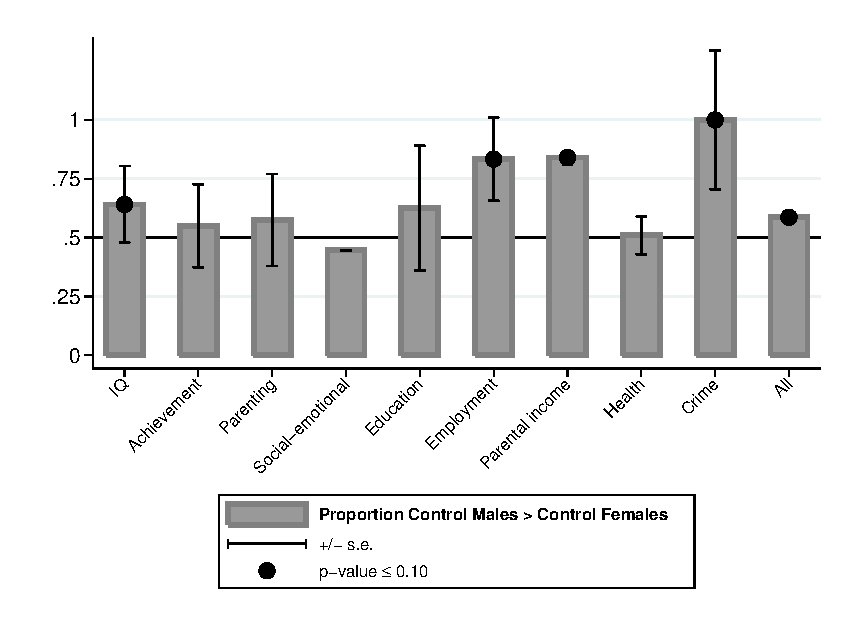
\includegraphics[width=\textwidth]{output/gendergaps-fullcontrol}
\end{subfigure}

\begin{subfigure}[h]{0.8\textwidth}
	\centering
	\caption{Treatment Gender Gaps}
	\label{fig:means-years}
	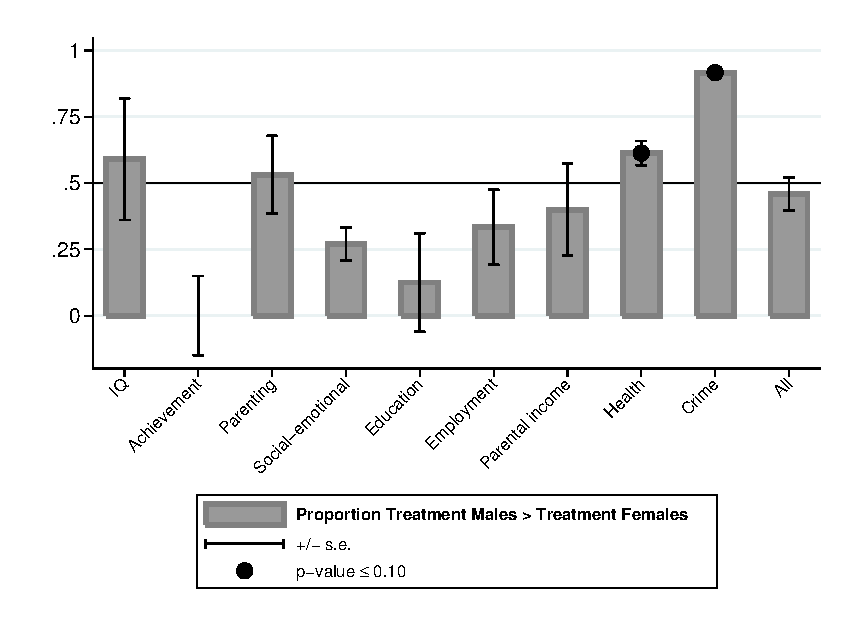
\includegraphics[width=\textwidth]{output/gendergaps-treatment}
\end{subfigure} 
\footnotesize \justify
Note: These plots show the proportion of outcomes, by outcome category, for which the males' mean is larger than the females' mean. The standard errors and the $p$-values are computed using 100 bootstraps. The $p$-values are one-sided and test the null hypothesis that the proportion of outcomes is greater than $\frac{1}{2}$ The crime outcomes are all coded so that a higher value indicates more criminal activity. All other outcome categories have higher values corresponding to socially desirable outcomes. 
\end{figure}

Table~\ref{tab:proportion-table} summarizes the gender gaps in these plots as well as those when considering the alternative setting of the control-group children. In the control group, the proportions of outcomes for which males do better than females is higher than $\frac{1}{2}$ for most of the categories, although by no means are all statistically significant. Exceptions include social-emotional skills, in which females surpass males, and crime, in which the outcomes are coded such that higher values correspond with less criminal activity. \textbf{[JJH: Code crime a positive!]} Treatment reverses the gaps for achievement, education, employment, parental income, and over all outcomes. It widens the gap for health, with treatment leading males to achieve better health outcomes. Considering control-group subjects who stay at home, females have better health outcomes and commit more crimes. Both outcomes are reduced with treatment \textbf{[JJH: Why worse health?]}. Finally, the males who attend lower-quality alternative preschools do not outperform females on any of the outcome categories associated with cognition, education, and parenting. This indicates an early-life disadvantage that enriched early childcare programs partially correct.

\begin{table}[H]
\centering
\caption{Summary of Proportion of Outcomes Males $>$ Females}
\label{tab:proportion-table}
\begin{threeparttable}
\begin{tabular}{l | c |c |c| c}
\toprule
& (1) & (2) & (3) & (4) \\
Category & Control Group  &  Control Group &  Control Group &  Treatment \\
	&				&	Stay at Home		& Alternative Preschool &  Group \\
\midrule  
IQ 								& \checkmark 	&  \checkmark* 		& $\times$	& \checkmark \\
Achievement						& \checkmark* 	&  \checkmark* 		&$\times$		& $\times$* \\
Social-emotional					& $\times$	& \checkmark 		&$\times$* 	&$\times$ \\
Parenting							& \checkmark	&  \checkmark* 		&$\times$ 	& $\times$ \\
Parental income					&  \checkmark  &\checkmark* 		& $\times$  	& \checkmark \\
Education							& \checkmark 	&\checkmark 		& $\times$ 	&	$\times$* \\
Employment						&  \checkmark* &  \checkmark* 		& $=$ 		&\checkmark* \\
Crime							&  $\times$* 	&  $=$ 			& $\times$* 	&  $\times$* \\
Risky Behavior						& $\times$	& $\times$*		& \checkmark	& $\times$* \\
Health 							& $=$ 		& $\times$ 		& $\times$ 	&  \checkmark *\\
Mental Health						& \checkmark* & \checkmark* 		&	\checkmark &	\checkmark \\

\midrule
All								&  \checkmark &\checkmark*&  $\times$ & $\times$\\
\bottomrule
\end{tabular}
\begin{tablenotes}
\footnotesize
\item Note: This table summarizes comparison of gender gaps across outcome categories by different groups. A checkmark indicates that the proportion of outcomes in the corresponding category is larger than $\frac{1}{2}$, meaning that males outperform females. A checkmark with an asterisk indicates that the proportion is significantly larger than $\frac{1}{2}$. Column (1) is the difference between males and females in the full control group.  Column (2) is the difference between males and females in the control group only considering those who stayed at home. Column (3) is the difference between males and females in the control group only considering those who attended alternative preschools. Column (4) is the difference between males and females in the treatment group.
\end{tablenotes}
\end{threeparttable}
\end{table}

Many studies have shown the potential for early-life interventions to improve the skills of children, especially those from disadvantaged families.\footnote{\citet{Currie_2011_AER,Elango_Hojman_etal_2016_Early-Edu}.} Several of these studies report effects by gender and find that males and females differently benefit from early childhood education. For example, \citet{Heckman_Moon_etal_2010_QE} and \citet{Garcia_Heckman_Leaf_etal_2017_Comp_CBA_Unpublished}, analyze randomized controlled trials with long-term data follow-ups, and find that intervening early in life more positively affects education for females and labor market and health outcomes for males. Other studies analyzing programs with shorter-term follow-up also find similar patterns of gender differences in early skills and academic outcomes.\footnote{\citet{Deming_2009_AEJAE,Ou_Reynolds_2010_Mechanisms_CYSR,Magnuson_Kelchen_Duncan_etal_2016_ECRQ}.} None of these studies have examined the gender gap and how treatment alters it.

This paper reports the treatment effects of ABC/CARE by gender. We report treatment effects comparing treated outcomes with different control conditions, including staying at home or attending other center-based care that was of lower quality than the ABC/CARE program.\footnote{Historical documentation, records, and evidence from knowledgeable individuals indicate that although these alternate centers followed state and federal standards, they were of lower quality than the ABC/CARE program.} Unlike previous studies, we compute treatment effects comparing the treatment group to the control group fixing those in the control group to these two alternate counterfactuals (shown in Figure 1?).\footnote{Previous studies presenting treatment effects of ABC and CARE include \citet{Ramey_etal_1985_Project-CARE_TiECSE, Clarke_Campbell_1998_ABC_Comparison_ECRQ,Campbell_Pungello_etal_2001_DP,Campbell_Ramey_etal_2002_ADS,Campbell_Wasik_etal_2008_ECRQ,Campbell_Conti_etal_2014_EarlyChildhoodInvestments}.}$^,$\footnote{See \cite{Heckman_1992_randomization}, \cite{Heckman_Hohmann_etal_2000_QJE}, and \cite{Kline_Walters_2016_QJE} for work related to control substitution.} Home care is beneficial for boys. 

This paper unfolds in the following way. In Section~\ref{sec:data}, we describe the experimental data and its special features. We document that a considerable proportion of the control group children attend lower (than treatment) preschools. In Sections~\ref{sec:parameters} and~\ref{sec:combining-functions} we define the treatment effects estimated. Section~\ref{sec:treatment-effects} reports the treatment effects overall and by gender and establish the existence of sharp gender effects in many categories of outcomes. Section~\ref{sec:gender-differences} discusses differences in the proportions of outcomes favoring men by category. Section~\ref{sec:conclusion} discusses the sources of these differences.


%ee \citet{Beeghly-etal_2017_IMHJ,Dayton_2017_IMHJ,Iruka_2017_IMHJ,Schore_2017_IMHJ} for recent findings on the topic of different development of males and females early in life. 	

\section{Background and Data}
\label{sec:data}
We analyze a combined sample of the two closely related interventions. Table~\ref{tab:abc-care-characteristics} summarizes the characteristics of the programs. Both interventions were implemented by researchers at the Frank Porter Graham Center at the University of North Carolina, Chapel Hill. ABC had four cohorts of subjects born between 1972 and 1977, and CARE had two cohorts of subjects born between 1978 and 1980. Both interventions targeted children from disadvantaged families in the Chapel Hill area. Eligibility was determined based on a High Risk Index (HRI) developed for ABC and minimally adapted for CARE.\footnote{See \citet{Campbell_Wasik_etal_2008_ECRQ}.} Example components of the HRI include father's presence, parental employment, and welfare receipt.\footnote{See Appendix~\ref{appendix:background} for the full HRI. \citet{Ramey_Smith_1977_AJMD, Wasik_Ramey_etal_1990_CD, Ramey_Campbell_1991_childreninpoverty}.}

Both interventions involved intensive center-based care for subjects in the treatment group starting at 8 weeks and continuing until age 5 before the children started kindergarten. Treatment-group subjects also received daily health screenings and diapers and formula until 6 months. Control-group families received the diapers and formula as well for the same period of time.\footnote{\citet{Wasik_Ramey_etal_1990_CD}.}  After school entrance up until age 8, there was an additional component of treatment in which home visitors worked with children and their parents to tutor the children and to encourage families to be involved in the children's academics.\footnote{In ABC, treatment status of this component was randomized. In CARE, all the subjects who received center-based care also received this school-age component.} We do not consider this part of the treatment because it extends beyond early childhood and in other work it was not found to have significant treatment effects.\footnote{\citet{Campbell_Ramey_etal_2002_ADS}.}

The pedagogical approach focused on language, cognitive, social-emotional, and executive functioning skills. During ABC and CARE, the \textit{Learning Games} curriculum was developed and refined.\footnote{\citet{Sparling_Lewis_1979_BOOKLearninggamesFirstThree}.} ABC and CARE subjects engaged with this in addition to other curricula that emphasized child-led learning of skills important for future learning.\footnote{\citet{Conti_etal_2016_LongTermHealth}.}

CARE included an additional arm of treatment. In addition to the services listed above, those in the treatment group received home visiting from birth to age 5. This home visiting consisted of biweekly visits focusing on parental problem solving skills. There was an additional experimental group that received this home visiting component, but not the center-based care.\footnote{\citet{Wasik_Ramey_etal_1990_CD}.} In light of previous analyses, we do not include this last group in our analysis. The home visiting component had weak effects.\footnote{\citet{Campbell_Conti_etal_2014_EarlyChildhoodInvestments} test for pooling.} We also use this lack of treatment effects to justify merging the treatment groups of ABC and CARE, even though that of CARE received the additional home-visiting component.\footnote{\citet{ABCCARE_Dataset}.}

\begin{table}[H]
\centering
\caption{ABC and CARE Program Overview}
\label{tab:abc-care-characteristics}
\begin{threeparttable}
	\begin{tabular}{l l}
	\toprule
Site & Chapel Hill, North Carolina \\
Cohorts & 4 (ABC), 2 (CARE) \\
$N$ & 58 treatment, 56 control (ABC) \\
	& 17 treatment, 23 control (CARE) \\
\midrule
Eligibility & HRI $>$ 11 \\
		& Biologically healthy \\
\midrule
Treatment years & 1972--1981 (ABC), 1977--1983 (CARE) \\
Treatment duration & 5 years \\
\midrule
Home visits 	& 2.5--2.7	per month (CARE)	\\
Center care	& 50	weeks per year \\
		 	& 30--45 hours per week  \\
Other treatment components & Formula until 6 months\\
					& Diapers until 6 months \\ 
					& Health check-ups \\
					& Medical care \\
					& Parenting instruction \\
					& Counseling \\
					& Transportation to center \\
Control-group incentives & Formula until 6 months \\
				& Diapers until 6 months 	\\
				& Health check-ups until 1 year (ABC, cohort 1) \\
\midrule
Adult-child ratio & 1:3--1:6 \\
Teacher requirements & High school through masters \\
				& Experience with children \\
Specialists & Physician, nurse, social worker \\
\bottomrule
\end{tabular}



\begin{tablenotes}
\footnotesize
\item Note: Characteristics that do not specify ABC or CARE were present in both. Biologically healthy includes lack of serious illness, including mental retardation. \\
\item Sources: \citet{Ramey_Collier_etal_1976_CarolinaAbecedarianProject,Ramey_Smith_1977_AJMD,Ramey_etal_1985_Project-CARE_TiECSE,Wasik_Ramey_etal_1990_CD,Ramey_Campbell_1991_childreninpoverty}.
\end{tablenotes}
\end{threeparttable}
\end{table}

Figure~\ref{fig:family-over-time} presents one aspect of family disadvantage.  The figure shows the evolution of the fathers' presence over time. At birth, there were few fathers present, especially for the females in the treatment group. This is a pattern commonly found in the literature. After birth, the proportion of fathers present, conditional being present at birth, remains stable.\footnote{For a more detailed description of the sample's disadvantage, see Appendix~\ref{appendix:background}.}

\begin{figure}[H]
\textbf{[JJH: Looks like a treatment effect on father present.][We report treatment effects on father present in Appendix C. There is a negative treatment effect for females between 3 and 5 years.}
\begin{center}
\caption{Father Present Over Time}
\label{fig:family-over-time}
		\label{fig:fhome}
			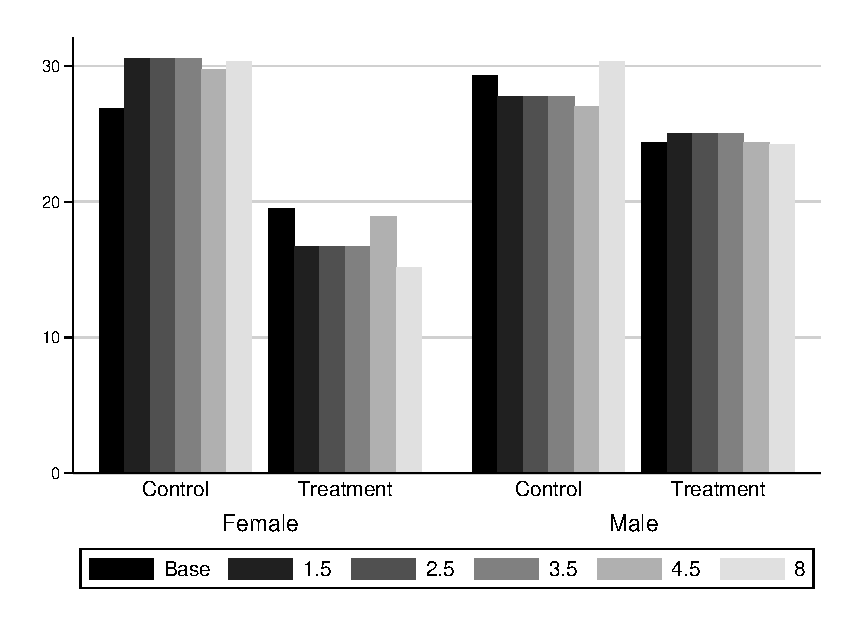
\includegraphics[width=0.65\textwidth]{output/family-fhome}
\end{center}
\footnotesize \justify
Note: The bars represent the proportion of father's presence. The bars after baseline are conditional on the father being at home at baseline.
\end{figure}

\subsection{Randomization Protocol and Compromises} \label{section:randomization}

Randomization for ABC/CARE was conducted on child pairs matched on family background. Siblings and twins were jointly randomized into either treatment or control groups.\footnote{For siblings, this occurred when two siblings were close enough in age such that both of them were eligible for the program.} Randomization pairing was based on a risk index, maternal education, maternal age, and gender of the subject.\footnote{We do not know the original pairs.} ABC collected an initial sample of 121 subjects. We characterize each missing observation in Appendix~\ref{appendix:background}.\footnote{In Appendix~\ref{appendix:estimates}, we document that our estimates are robust when we adjust for missing data using standard weighting (matching) methods described in Appendix~\ref{app:method_partialobs}.} We conduct the same analysis for the CARE sample. 22 subjects in ABC did not stay in the program through age 5. Dropouts are evenly balanced and are primarily related to the health of the child and mobility of families and not to dissatisfaction with the program.\footnote{The 22 dropouts include four children who died, four children who left the study because their parents moved, and two children who were diagnosed as developmentally delayed. Details are in Table~\ref{table:abccompromises}. Everyone offered the program was randomized to either treatment or control. All eligible families agreed to participate. Dropping out occurs \emph{after} randomization.}

\subsection{Control Group Substitution}

In ABC/CARE, many control-group subjects (but no treatment-group subjects) attended alternative center-based preschool.\footnote{See \cite{Heckman_Hohmann_etal_2000_QJE} on the issue of substitution bias in social experiments.} The figure is \treatsubsabc\ for ABC and \treatsubscarec\ for CARE. This creates both a problem (substitution bias\footnote{See \cite{Heckman_1992_randomization}, \cite{Heckman_Hohmann_etal_2000_QJE}, and \cite{Kline_Walters_2016_QJE}.}) and an opportunity (we can compare the effect of an enriched treatment vs. other alternative home and low quality environments). We discuss both.

\begin{sidewaysfigure}[!htbp]
\centering
\caption{Control Substitution Characteristics, ABC/CARE Control Group}\label{fig:control-sub}
\begin{subfigure}[h]{0.49\textwidth}
	\centering
	\caption{Cumulative Enrollment} \label{fig:treatsubcare}
	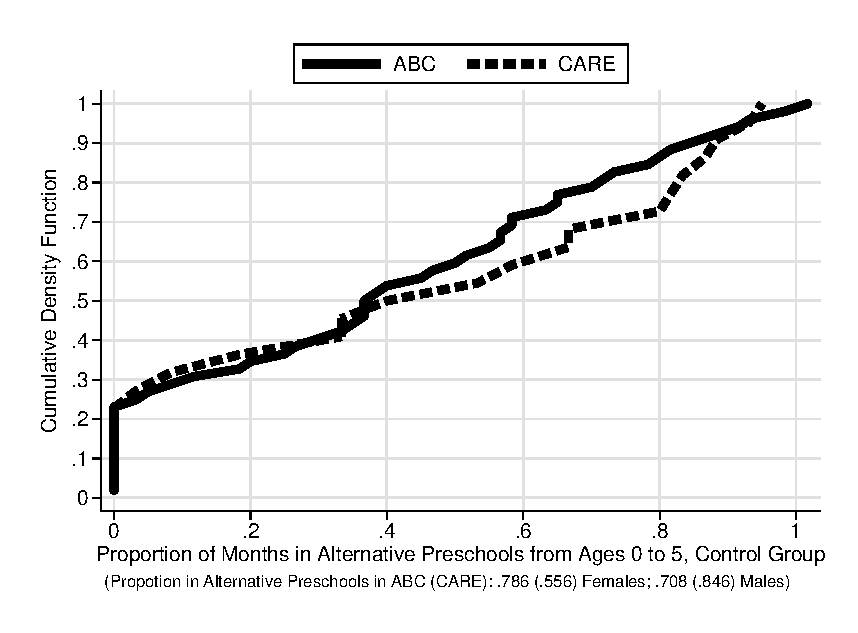
\includegraphics[width=\textwidth]{output/abccare_controlcontamination.eps}
\end{subfigure}
\begin{subfigure}[h]{0.49\textwidth}
	\centering
	\caption{Enrollment Dynamics} \label{fig:proportion-alt-pre}
	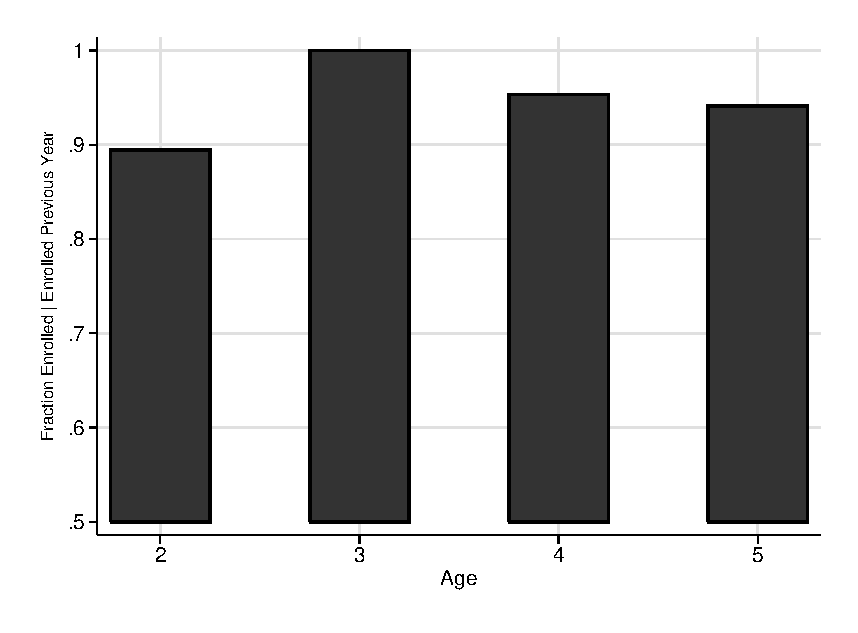
\includegraphics[width=\textwidth]{output/abccare_Vprobs.eps}
\end{subfigure}%
\footnotesize \justify
Note: Panel (a) displays the cumulative distribution function of enrollment in alternatives. Panel (b) displays the fraction of ABC/CARE control-group children enrolled in alternatives, conditional on being enrolled in the previous age (at least one month).\\
\end{sidewaysfigure}

Figure~\ref{fig:treatsubcare} shows the cumulative distribution of the proportion of time in the first five years that control subjects were enrolled in alternatives. Figure~\ref{fig:proportion-alt-pre} shows the dynamics of enrollment. Those who enroll generally stay enrolled. As control children age, they are more likely to enter childcare (see Appendix~\ref{app:control-subbb}).

Children in the control group who are enrolled in alternative early childcare programs are less economically disadvantaged at baseline compared to children who stay at home. Disadvantage is measured by maternal education, maternal IQ, Apgar scores, and the high-risk index defining ABC/CARE eligibility. Children who attend alternatives have fewer siblings. On average, they are children of mothers who are more likely to be working at baseline.\footnote{Statistically significant at 10\%.} Parents of girls are much more likely to use alternative childcare if assigned to the control group.\footnote{See Table~\ref{table:controlsubscharacteristics} in Appendix~\ref{appendix:background} for tests of differences across these variables between children in the control group who attended and who did not attend alternative preschools.} If a boy, father more likely present.

While most of the alternative childcare centers received federal subsidies and were subject to the federal regulations of the era, they were relatively low quality compared to ABC/CARE.\footnote{Appendix~\ref{appendix:tetanus} discusses the federal standards of that day. See \citet{Department-of-Health_1968_DayCareRequirements,NCGA_1971_House-Bill-100,Ramey-et-al_1977_Intro-to-ABC,Ramey_Campbell_1979_SR,Ramey_McGinness_etal_1982_Abecedarianapproach, Burchinal_Campbell_etal_1997_CD}.}$^,$\footnote{When we compare ABC/CARE treatment to these alternatives, ABC/CARE has substantial treatment effects. Further, as we argue below, parents perceived that ABC/CARE was superior to the alternatives.} The access of control-group children to alternative programs affects the interpretation of estimated treatment effects, as we discuss next.


\section{Parameters Estimated in This Paper} 
\label{sec:parameters}
Random assignment to treatment does not guarantee that conventional treatment effect estimators answer policy-relevant questions. We define and estimate three parameters that address different policy questions.

Let $W=1$ indicate that the parents referred to the program participate in the randomization protocol. $W=0$ indicates otherwise. $R$ indicates randomization into the treatment group ($R = 1$) or to the control group ($R = 0$). $D$ indicates attending the program, i.e., $D = R$ implies compliance with the initial randomization protocol.

Individuals are eligible to participate in the program if baseline background variables $\bm{B}\in\mathcal{B}_0$. $\mathcal{B}_0$ is the set of scores on the risk index that determines program eligibility. Because all of the eligible people given the option to participate choose to do so $(W=1\text{ and } D=R)$, we can safely interpret the treatment effects generated by the experiment as average treatment effects for the population for which $\bm{B}\in\mathcal{B}_0$ and not just treatment effects for the treated.\footnote{According to \citet{Ramey_Yeates_Short_1984_CD}, there was only one eligible mother who refused to participate in the randomization.}

Let $Y^1_{j}$ be the outcome $j$ for the treated, and $Y^0_{j}$ be the control counterfactual. $Y^0_{j}$ depends on the exposure to various alternative preschools while ABC/CARE was active (i.e.,\ it depends on the degree of control substitution).\footnote{This is an example of control-group subjects of a social experiment finding a treatment substitute. See \cite{Heckman_Hohmann_etal_2000_QJE} for methodological solutions and an example of implementation.} The index set for the outcomes is $\mathcal{J}$, which we can partition by age (\ $\mathcal{J}_a$ with $\mathcal{J} = \bigcup \limits _{a \in \mathcal{A}} \mathcal{J}_a$ and $\mathcal{A}$ indexes age) or by outcome category (\ $\mathcal{J}_\ell$ with $\mathcal{J} = \bigcup \limits _{\ell \in \mathcal{L}} \mathcal{J}_\ell$ and $\mathcal{L}$ indexes categories).

All treatment-group children had the same exposure to the ABC/CARE treatment and no exposure to alternative center-based care.\footnote{We discuss cases of attrition during the program in Appendix~\ref{appendix:background}.} It would be desirable to identify and estimate parameters evaluating ABC/CARE against all possible levels of exposure to alternative preschools, but our samples are too small to credibly do so. We simplify the analysis of the counterfactual to ABC/CARE by creating two categories. ``$H$'' indicates that the control-group child stays at home throughout the entire length of the program. ``$C$'' indicates that a control-group child is in alternative center childcare for any amount of time.\footnote{This categorization is consistent with Figure~\ref{fig:proportion-alt-pre}. Once parents decided to enroll their children in alternative preschools, the children tended to stay enrolled up to age 5.} We test the sensitivity of our estimates to the choice of different categorizations in our empirical analysis in Appendix~\ref{appendix:vsensitivity-controlsub}. We thus compress a complex reality into two counterfactual outcome states for each outcome $j$:
\begin{align*}
Y_{j,H}^0 \quad &: \quad \textbf{ Subject received home care exclusively} \\
Y_{j,C}^0 \quad &: \quad \textbf{ Subject attended some alternative preschool}.
\end{align*}


One parameter of interest addresses the question: What is the effect of the program as implemented? This is the effect of the program compared to the next best alternative as perceived by the parents (or the relevant decision maker) and is defined by
\begin{equation}\label{eq:effect}
\Delta_j := \mathbb{E} \left[ Y_{j}^1 -  Y_{j}^0 | W =1 \right] = \mathbb{E} \left[Y_{j}^1 -  Y_{j}^0 | \bm{B} \in \mathcal{B}_0 \right],
\end{equation}
where the second equality follows because everyone who was eligible elected to participate in the program. For the sample of eligible people, this parameter addresses the effectiveness of the program relative to the quality of all available alternatives when the program was implemented, including staying at home. This is the Local Average Treatment Effect (LATE).\footnote{\citet{Imbens_Angrist_1994_Econometrica}.}

We define $V$ as a dummy variable indicating that the control-group child attended alternative center-based childcare. $V=0$ denotes that the control-group child stayed at home. The outcome when a child is in the control group is
\begin{equation}
Y_{j}^0 : = \left( 1 - V \right) Y_{j,H}^0 + \left( V \right) Y_{j,C}^0. \label{eq:meandiff}
\end{equation}
\noindent It is fruitful to assess the effectiveness of the program compared to a world in which the child stays at home full time. The associated causal parameter is:
\begin{equation}\label{eq:cont1}
\Delta_j \left(\text{\textbf{Fix }}V = 0 \right) : =   \mathbb{E} \left[ Y_{j}^1 -  Y_{j}^0 | \text{\textbf{Fix }}V = 0, W = 1 \right] := \mathbb{E} \left[Y_{j}^1 -  Y_{j}^0 | \text{\textbf{Fix }}V = 0, \bm{B} \in \mathcal{B}_0 \right].
\end{equation}
It is also useful to assess the average effectiveness of a program relative to attending an alternative preschool with associated causal parameter:
\begin{equation}\label{eq:cont2}
\Delta_j \left( \text{\textbf{Fix }} V =1 \right) : =   \mathbb{E} \left[ Y_{j}^1 -  Y_{j}^0 | \text{\textbf{Fix }} V = 1, W = 1 \right] := \mathbb{E} \left[ Y_{j}^1 -  Y_{j}^0 | \text{\textbf{Fix }} V = 1, \bm{B} \in \mathcal{B}_0 \right].
\end{equation}

\noindent ``\textbf{Fix}'' means $V$ is fixed to the designated value.\footnote{For the distinction between fixing and conditioning, see \citet{Haavelmo_1943_Econometrica} and \citet{Heckman_Pinto_2015_EconometTheory}.}

Random assignment to treatment does not directly identify the parameters in Equations~\eqref{eq:cont1} or~\eqref{eq:cont2}. Econometric methods are required. In this paper, we rely on matching to control for selection into home or an alternative preschool by the control group. We assume that observed characteristics are sufficient to describe the selection into alternative center-based arrangements. In Appendix~\ref{appendix:results}, we show the balance across the groups in the matched samples along the observed selection variables (e.g., family characteristics, Apgar scores, gender), further justifying this approach.\footnote{To select adequate variables for matching, we conduct goodness of fit tests to find the most predictive set of baseline characteristics subject to penalty for adding parameters. This procedure is fully explained in Appendix~\ref{appendix:results}.}

We report estimates from alternative empirical strategies, including instrumental variables and control functions, in Appendix~\ref{appendix:amethodology}. The estimates from these alternative estimation strategies are consistent with results from matching but lack precision. Appendix~\ref{appendix:vsensitivity-controlsub} displays results with alternative definitions of $V$ (i.e., different thresholds define if a child attended alternative preschool). The results are robust to the various definitions. What matters is whether any center-based child care is being used ($V>0$)---not the specific value of $V$.

\subsection{Summarizing Multiple Treatment Effects}\label{sec:combining-functions}

The extensive data for ABC/CARE generates many outcomes that we can use to evaluate the program. Summarizing these effects in an interpretable way is challenging.\footnote{In Appendix~\ref{appendix:results} we present an exhaustive list of treatment effects correcting the $p$-values using the step-down procedure in \citet{Romano_Wolf_2016_pval_SaPL}.} We present effect sizes averaged over outcomes. We also construct combining functions that count the proportion of treatment effects that are positive for different categories of outcomes. Similarly, we study the count of the proportion of treatment effects that are positive and statistically significant at the 10\% level. We complement these analyses by applying an exact non-parametric test on the equality of the distributions of outcomes across treatment groups developed in \citet{Rosenbaum_2005_Distribution_JRSS}.

\textbf{Combining Functions.} Consider a block of outcomes $\mathcal{J}_{\ell}, \ell \in \{1,\dots ,L\}$, with cardinality $B_{\ell}$ and  associated treatment effects $\Delta_1, \ldots \Delta_{B_\ell}$. We assume that outcomes can be ordered so that $\Delta_{j} >0$ is beneficial.\footnote{All but 5\% of the outcomes we study can be ranked in this fashion. See Appendix~\ref{appendix:results} for a discussion.} The count of positive treatment effects within block $\mathcal{J}_{\ell}$ is:
\begin{equation}
C_\ell = \sum^{B_\ell}_{j=1} \bm{1} (\Delta_{j} >0),
\end{equation}

\noindent The proportion of beneficial outcomes, our combining function, is $C_\ell / B_\ell$. In our empirical application we consider all the outcomes as a block. Different blocks are grouped by age (e.g.,\ childhood, school age, adulthood) or by common categories (e.g.,\ employment, health, crime).

Under the null hypothesis of no treatment effect for the block of outcomes indexed by $\mathcal{J}_\ell$, and assuming the validity of asymptotic approximations, $C_\ell / B_\ell$ is centered at $\frac{1}{2}$.\footnote{\citet{Campbell_Conti_etal_2014_EarlyChildhoodInvestments} establish a validity of asymptotic approximations for the ABC sample.} We compute the fraction $C_\ell / B_\ell$ and the corresponding bootstrapped empirical distribution to obtain a $p$-value. The bootstrap procedure accounts for dependence in unobservables across outcomes (within blocks) in a general way.

Our test based on the number of outcomes for which the treatment effect is statistically significant at the $10\%$ level produces similar inference. Under the null hypothesis, 10\% of all outcomes should be ``significant'' at the 10\% level even if there is no treatment effect of the program.\footnote{In this case, we perform a ``double bootstrap'' procedure to first determine significant treatment effects at $10\%$ level and then calculate the standard error of the count.} The combining functions avoid: (i) arbitrarily picking outcomes that have statistically significant effects---``cherry picking''; or (ii) arbitrarily selecting blocks of outcomes to correct the $p$-values when accounting for multiple hypothesis testing. We present $p$-values for these hypotheses and a number of combining functions by outcome category in Appendix~\ref{appendix:results}.\footnote{In Appendix~\ref{appendix:results}, we present yet another alternative. We calculate a latent measure, using principal component analysis, of the set of outcomes within a block and perform inference on this latent measure. This analysis also points to beneficial effects of the program.}

\textbf{An Exact Non-Parametric Test.} We also test for equality of treatment and control distributions by outcome using an exact test developed by \citet{Rosenbaum_2005_Distribution_JRSS}. We provide a brief explanation of the test and refer interested readers to the original source for more details. Let $\mathcal{N}$ index the individuals in our sample and consider the block of outcomes $\mathcal{J}_\ell$. Let $d_{ii'}$ be the distance between the individuals $i, i' \in \mathcal{N}$, $i \neq i'$, based on the outcomes in $\mathcal{J}_\ell$. In our application, this is the Mahalanobis distance.\footnote{\citet{Mahalanobis_1936_PNISI}.} There is an optimal non-bipartite pairing of individuals according to $d_{ii'}$.\footnote{\citet{Derigs_1988_Solving_AOR}.} This is obtained by minimizing the distance across all possible pairings $i, i'$ in the sample.

Under the null hypothesis of no treatment effects, pairings of treatment-group children with control-group children should be as frequent as pairings of treatment-group children with other treatment-group children and control-group children with other control-group children. If a relatively large number of pairs are matched equally across groups using this metric, we fail to reject the null hypothesis that the joint distribution of outcomes in block $\mathcal{J}_{\ell}, \ell \in \{1,\dots ,L\}$ is the same across the treatment and control groups.

The number of treatment-control pairings in the optimal non-bipartite pairing within the block of outcomes $\mathcal{J}_\ell$, denoted by $A_{\ell}, \ell \in \{1,\dots ,L\}$, is a summary statistic allowing us to test the null hypothesis of interest. Its exact $p$-value can be calculated. Asymptotically, the studentized value of $A_\ell$ follows a normal standard distribution. For each block, we present these asymptotic $p$-values to complement the information provided by the combining functions.\footnote{The exact $p$-values render similar results. We display the asymptotic $p$-values for expositional simplicity.}


\section{Summarizing Multiple Treatment Effects}
\label{sec:combining-functions}
ABC/CARE has rich longitudinal data on multiple outcomes over multiple periods of the life cycle. Summarizing these effects in an interpretable way is challenging.\footnote{Appendix~\ref{appendix:results} presents step-down $p$-values for the blocks of outcomes that are used in our benefit/cost analysis which we summarize in this section (\citealp{Lehman_Romano_2005_AnnStat} and \citealp{Romano_Shaikh_2006_AnnStat}). We follow the algorithm in \citet{Romano_Wolf_2016_pval_SaPL}.} Simpler, more digestible summary measures are useful for understanding our main findings. This section discusses our approach to summarizing vectors of treatment effects using combining functions that count the proportion of treatment effects that are positive by different categories of outcomes.

Consider a block of $N_l$ outcomes indexed by set $Q_l = \{1,\dots,N_l\}$. Let $j \in Q_l$ be a particular outcome within block $l$. Associated with it is a mean treatment effect
\begin{equation}
\Delta_{j,a} : = \mathbb{E} \left[ Y^1_{j,a} - Y^0_{j,a} | \bm{B} \in \mathcal{B}_0 \right], j \in Q_l.
\end{equation}

We assume that outcomes can be ordered so that $\Delta_{j,t} >0$ is beneficial.\footnote{All but 5\% of the outcomes we study can be ranked in this fashion. See Appendix~\ref{appendix:results} for a discussion.} We summarize the estimated effects of the program on outcomes within the block by the count of positive impacts within block $l$:
\begin{equation}
C_l = \sum^{N_l}_{j=1} 1 (\hat{\Delta}_{j,a} >0).
\end{equation}
The proportion of beneficial outcomes in block $l$ is $C_l / N_l$.\footnote{In our empirical application we consider all the outcomes as a block, and then different blocks grouped according to common categories---e.g., skills, health, crime.}

Let $\mathcal{L}$ be the set of blocks. Under the null hypothesis of no treatment effects for all $j \in Q_l, l \in \mathcal{L}$, and assuming the validity of asymptotic approximations, $C_l / N_l$ should be centered around $\frac{1}{2}$. We bootstrap to obtain $p$-values for the null for each block and over all blocks. This procedure accounts for dependence in unobservables across outcomes and for pretesting.\footnote{Bootstrapping allows us to account for dependence across outcomes in a general way.} We also count the beneficial treatment effects that are statistically significant in the sets of outcomes across each of the groups indexed by the set $Q_l$. Using a 10\% significance level, on average 10\% of all outcomes should be ``significant'' at the 10\% level even if there is no treatment effect of the program. We provide evidence against both null hypotheses.\footnote{In this case, we perform a ``double bootstrap'' procedure to first determine significant treatment effects at $10\%$ level and then calculate the standard error of the count.} Combining counts across all blocks enables us to avoid (i) arbitrarily picking outcomes that have statistically significant effects---``cherry picking''; or (ii) arbitrarily selecting blocks of outcomes to correct the $p$-values when accounting for multiple hypothesis testing.\footnote{We present $p$-values for these hypotheses and a number of combining functions by outcome category in Appendix~\ref{appendix:results}.}$^{\text{,}}$\footnote{In Appendix~\ref{appendix:results} we present yet another alternative. We calculate a ``latent'' outcome out of the set of outcomes within a block and perform inference on this latent. The results point to beneficial effects of the program in this case as well.}


\section{Treatment Effects}
\label{sec:treatment-effects}
\subsection{Estimated Treatment Effects}

Tables~\ref{table:tescombinedmales} and \ref{table:tescombinedfemales} present the estimates of selected treatment effects for males and females respectively. The complete set of treatment effects are listed in Appendix~\ref{appendix:results}. Column (1) gives sample mean differences in outcomes between treatment and control groups. Column (2) adjusts the differences for attrition and controls for background variables. Both are estimates of the parameter defined in equation~\eqref{eq:effect}. Column (3) shows the mean difference between the full treatment-group and the control-group subjects who did not attend alternative preschools. Column (4) gives standard matching estimates for the parameter defined in equation~\eqref{eq:influenza}.\footnote{In Appendix~\ref{app:matching-is-fun}, we provide details on: (i) the kernel matching estimator that we use; (ii) the matching variables that we use; and (iii) a sensitivity analysis to these matching variables.} Column (5) gives mean differences between the full treatment-group and control-group children who attended alternatives. Column (6) gives matching estimates for the parameter of equation~\eqref{eq:smallpox}.

The results for females show that ABC/CARE has substantial effects on education when comparing outcomes of the treatment-group subjects to those from the next best alternative. High school graduation increases between 13 and 25 percentage points, depending on the estimate that we consider; college graduation increases 13 percentage points; and the average years of schooling increase between 2.1 and 1.8 years. Employment at age 30 increases between 13 and 8 percentage points. ABC/CARE has substantial impacts on human capital accumulation and employment. The results strengthen when we compare treatment with the option of staying at home.

\textbf{[JJH: Let's be more precise: show by category. Put this in the main text.][Step down $p$-values are now reported in Tables~\ref{table:tescombinedmales} and \ref{table:tescombinedfemales} in the square brackets.]}

\begin{sidewaystable}[!htbp]
\centering
\begin{threeparttable}
\caption{Treatment Effects on Selected Outcomes, Males}\label{table:tescombinedmales}
\begin{scriptsize}
  \begin{tabular}{cccccccccccc}
  \toprule
   Category & Variable & Age & $\bar{Y}_C$ & (1) & (2) & (3) & (4) & (5) & (6) \\

    \midrule
    % cat 3
     \mc{1}{l}{\scriptsize{Parental Income}} &   \mc{1}{l}{\scriptsize{Parental Labor Income}} & \mc{1}{c}{\scriptsize{3.5}} & \mc{1}{c}{\scriptsize{13,505}} & \mc{1}{c}{\scriptsize{1,036}} & \mc{1}{c}{\scriptsize{494}} & \mc{1}{c}{\scriptsize{73.862}} & \mc{1}{c}{\scriptsize{1,462}} & \mc{1}{c}{\scriptsize{123}} & \mc{1}{c}{\scriptsize{690}} \\  

  &   &  & & \mc{1}{c}{\scriptsize{(0.374)}} & \mc{1}{c}{\scriptsize{(0.411)}} & \mc{1}{c}{\scriptsize{(0.474)}} & \mc{1}{c}{\scriptsize{(0.390)}} & \mc{1}{c}{\scriptsize{(0.479)}} & \mc{1}{c}{\scriptsize{(0.417)}} \\  

  &   & \mc{1}{c}{\scriptsize{12}} & \mc{1}{c}{\scriptsize{23,868}} & \mc{1}{c}{\scriptsize{7,085}} & \mc{1}{c}{\scriptsize{9,625}} & \mc{1}{c}{\scriptsize{18,050}} & \mc{1}{c}{\scriptsize{12,639}} & \mc{1}{c}{\scriptsize{6,620}} & \mc{1}{c}{\scriptsize{5,383}} \\  

  &   &  & & \mc{1}{c}{\scriptsize{\textbf{(0.092)}}} & \mc{1}{c}{\scriptsize{\textbf{(0.020)}}} & \mc{1}{c}{\scriptsize{\textbf{(0.038)}}} & \mc{1}{c}{\scriptsize{\textbf{(0.074)}}} & \mc{1}{c}{\scriptsize{\textbf{(0.098)}}} & \mc{1}{c}{\scriptsize{(0.139)}} \\  

  &   & \mc{1}{c}{\scriptsize{15}} & \mc{1}{c}{\scriptsize{22,985}} & \mc{1}{c}{\scriptsize{8,488}} & \mc{1}{c}{\scriptsize{4,495}} & \mc{1}{c}{\scriptsize{5,540}} & \mc{1}{c}{\scriptsize{4,805}} & \mc{1}{c}{\scriptsize{2,885}} & \mc{1}{c}{\scriptsize{4,345}} \\  

  &   &  & & \mc{1}{c}{\scriptsize{\textbf{(0.071)}}} & \mc{1}{c}{\scriptsize{(0.221)}} & \mc{1}{c}{\scriptsize{(0.243)}} & \mc{1}{c}{\scriptsize{(0.264)}} & \mc{1}{c}{\scriptsize{(0.354)}} & \mc{1}{c}{\scriptsize{(0.296)}} \\  

  &   & \mc{1}{c}{\scriptsize{21}} & \mc{1}{c}{\scriptsize{21,585}} & \mc{1}{c}{\scriptsize{12,732}} & \mc{1}{c}{\scriptsize{8,809}} & \mc{1}{c}{\scriptsize{122}} & \mc{1}{c}{\scriptsize{-933}} & \mc{1}{c}{\scriptsize{10,784}} & \mc{1}{c}{\scriptsize{10,283}} \\  

  &   &  & & \mc{1}{c}{\scriptsize{\textbf{(0.005)}}} & \mc{1}{c}{\scriptsize{\textbf{(0.098)}}} & \mc{1}{c}{\scriptsize{(0.448)}} & \mc{1}{c}{\scriptsize{(0.456)}} & \mc{1}{c}{\scriptsize{\textbf{(0.056)}}} & \mc{1}{c}{\scriptsize{\textbf{(0.041)}}} \\  

   \mc{1}{l}{\scriptsize{Education}} &   \mc{1}{l}{\scriptsize{Graduated High School}} & \mc{1}{c}{\scriptsize{30}} & \mc{1}{c}{\scriptsize{0.600}} & \mc{1}{c}{\scriptsize{0.073}} & \mc{1}{c}{\scriptsize{0.044}} & \mc{1}{c}{\scriptsize{0.116}} & \mc{1}{c}{\scriptsize{0.083}} & \mc{1}{c}{\scriptsize{0.040}} & \mc{1}{c}{\scriptsize{0.063}} \\  

  &   &  & & \mc{1}{c}{\scriptsize{(0.262)}} & \mc{1}{c}{\scriptsize{(0.375)}} & \mc{1}{c}{\scriptsize{\textbf{(0.001)}}} & \mc{1}{c}{\scriptsize{(0.346)}} & \mc{1}{c}{\scriptsize{(0.407)}} & \mc{1}{c}{\scriptsize{(0.317)}} \\  

  &  \mc{1}{l}{\scriptsize{Graduated 4-year College}} & \mc{1}{c}{\scriptsize{30}} & \mc{1}{c}{\scriptsize{0.120}} & \mc{1}{c}{\scriptsize{0.170}} & \mc{1}{c}{\scriptsize{0.138}} & \mc{1}{c}{\scriptsize{0.149}} & \mc{1}{c}{\scriptsize{0.099}} & \mc{1}{c}{\scriptsize{0.135}} & \mc{1}{c}{\scriptsize{0.143}} \\  

  &   &  & & \mc{1}{c}{\scriptsize{\textbf{(0.055)}}} & \mc{1}{c}{\scriptsize{(0.128)}} & \mc{1}{c}{\scriptsize{(0.216)}} & \mc{1}{c}{\scriptsize{(0.338)}} & \mc{1}{c}{\scriptsize{(0.154)}} & \mc{1}{c}{\scriptsize{(0.130)}} \\  

  &  \mc{1}{l}{\scriptsize{Years of Education}} & \mc{1}{c}{\scriptsize{30}} & \mc{1}{c}{\scriptsize{12.867}} & \mc{1}{c}{\scriptsize{0.525}} & \mc{1}{c}{\scriptsize{0.541}} & \mc{1}{c}{\scriptsize{1.010}} & \mc{1}{c}{\scriptsize{0.777}} & \mc{1}{c}{\scriptsize{0.351}} & \mc{1}{c}{\scriptsize{0.344}} \\  

  &   &  & & \mc{1}{c}{\scriptsize{(0.151)}} & \mc{1}{c}{\scriptsize{(0.163)}} & \mc{1}{c}{\scriptsize{(0.998)}} & \mc{1}{c}{\scriptsize{(0.136)}} & \mc{1}{c}{\scriptsize{(0.280)}} & \mc{1}{c}{\scriptsize{(0.256)}} \\  

   \mc{1}{l}{\scriptsize{Labor Income}} &   \mc{1}{l}{\scriptsize{Employed}} & \mc{1}{c}{\scriptsize{30}} & \mc{1}{c}{\scriptsize{0.700}} & \mc{1}{c}{\scriptsize{0.119}} & \mc{1}{c}{\scriptsize{0.196}} & \mc{1}{c}{\scriptsize{0.108}} & \mc{1}{c}{\scriptsize{0.040}} & \mc{1}{c}{\scriptsize{0.237}} & \mc{1}{c}{\scriptsize{0.261}} \\  

 &    &  & & \mc{1}{c}{\scriptsize{(0.128)}} & \mc{1}{c}{\scriptsize{\textbf{(0.025)}}} & \mc{1}{c}{\scriptsize{\textbf{(0.001)}}} & \mc{1}{c}{\scriptsize{(0.383)}} & \mc{1}{c}{\scriptsize{\textbf{(0.025)}}} & \mc{1}{c}{\scriptsize{\textbf{(0.013)}}} \\  

  &  \mc{1}{l}{\scriptsize{Labor Income}} & \mc{1}{c}{\scriptsize{30}} & \mc{1}{c}{\scriptsize{30,079}} & \mc{1}{c}{\scriptsize{19,810}} & \mc{1}{c}{\scriptsize{24,365}} & \mc{1}{c}{\scriptsize{25,220}} & \mc{1}{c}{\scriptsize{20,611}} & \mc{1}{c}{\scriptsize{23,072}} & \mc{1}{c}{\scriptsize{21,836}} \\  

   &  &  & & \mc{1}{c}{\scriptsize{\textbf{(0.091)}}} & \mc{1}{c}{\scriptsize{\textbf{(0.092)}}} & \mc{1}{c}{\scriptsize{(0.998)}} & \mc{1}{c}{\scriptsize{(0.122)}} & \mc{1}{c}{\scriptsize{(0.107)}} & \mc{1}{c}{\scriptsize{\textbf{(0.094)}}} \\  

  \mc{1}{l}{\scriptsize{Crime}} &    \mc{1}{l}{\scriptsize{Total Felony Arrests}} & \mc{1}{c}{\scriptsize{Mid-30s}} & \mc{1}{c}{\scriptsize{1.370}} & \mc{1}{c}{\scriptsize{0.196}} & \mc{1}{c}{\scriptsize{0.685}} & \mc{1}{c}{\scriptsize{1.523}} & \mc{1}{c}{\scriptsize{1.340}} & \mc{1}{c}{\scriptsize{0.481}} & \mc{1}{c}{\scriptsize{0.188}} \\  

   &  &  & & \mc{1}{c}{\scriptsize{(0.368)}} & \mc{1}{c}{\scriptsize{(0.183)}} & \mc{1}{c}{\scriptsize{\textbf{(0.064)}}} & \mc{1}{c}{\scriptsize{\textbf{(0.026)}}} & \mc{1}{c}{\scriptsize{(0.284)}} & \mc{1}{c}{\scriptsize{(0.410)}} \\  

  &  \mc{1}{l}{\scriptsize{Total Misdemeanor Arrests}} & \mc{1}{c}{\scriptsize{Mid-30s}} & \mc{1}{c}{\scriptsize{1.296}} & \mc{1}{c}{\scriptsize{-0.501}} & \mc{1}{c}{\scriptsize{-0.244}} & \mc{1}{c}{\scriptsize{-0.298}} & \mc{1}{c}{\scriptsize{-0.034}} & \mc{1}{c}{\scriptsize{-0.246}} & \mc{1}{c}{\scriptsize{-0.507}} \\  

  &   &  & & \mc{1}{c}{\scriptsize{(0.171)}} & \mc{1}{c}{\scriptsize{(0.289)}} & \mc{1}{c}{\scriptsize{(0.314)}} & \mc{1}{c}{\scriptsize{(0.422)}} & \mc{1}{c}{\scriptsize{(0.329)}} & \mc{1}{c}{\scriptsize{(0.168)}} \\  

   \mc{1}{l}{\scriptsize{Health}} &   \mc{1}{l}{\scriptsize{Self-reported drug user}} & \mc{1}{c}{\scriptsize{Mid-30s}} & \mc{1}{c}{\scriptsize{0.500}} & \mc{1}{c}{\scriptsize{-0.333}} & \mc{1}{c}{\scriptsize{-0.438}} & \mc{1}{c}{\scriptsize{-0.673}} & \mc{1}{c}{\scriptsize{-0.557}} & \mc{1}{c}{\scriptsize{-0.326}} & \mc{1}{c}{\scriptsize{-0.330}} \\  

   &  &  & & \mc{1}{c}{\scriptsize{\textbf{(0.019)}}} & \mc{1}{c}{\scriptsize{\textbf{(0.002)}}} & \mc{1}{c}{\scriptsize{\textbf{(0.000)}}} & \mc{1}{c}{\scriptsize{\textbf{(0.000)}}} & \mc{1}{c}{\scriptsize{\textbf{(0.039)}}} & \mc{1}{c}{\scriptsize{\textbf{(0.023)}}} \\  

  &  \mc{1}{l}{\scriptsize{Systolic Blood Pressure (mm Hg)}} & \mc{1}{c}{\scriptsize{Mid-30s}} & \mc{1}{c}{\scriptsize{138.071}} & \mc{1}{c}{\scriptsize{-9.791}} & \mc{1}{c}{\scriptsize{-13.275}} & \mc{1}{c}{\scriptsize{14.196}} & \mc{1}{c}{\scriptsize{14.976}} & \mc{1}{c}{\scriptsize{-24.166}} & \mc{1}{c}{\scriptsize{-18.559}} \\  

  &   &  & & \mc{1}{c}{\scriptsize{(0.113)}} & \mc{1}{c}{\scriptsize{\textbf{(0.049)}}} & \mc{1}{c}{\scriptsize{\textbf{(0.013)}}} & \mc{1}{c}{\scriptsize{\textbf{(0.000)}}} & \mc{1}{c}{\scriptsize{\textbf{(0.000)}}} & \mc{1}{c}{\scriptsize{\textbf{(0.011)}}} \\  

  &  \mc{1}{l}{\scriptsize{Diastolic Blood Pressure (mm Hg)}} & \mc{1}{c}{\scriptsize{Mid-30s}} & \mc{1}{c}{\scriptsize{89.214}} & \mc{1}{c}{\scriptsize{-10.854}} & \mc{1}{c}{\scriptsize{-14.134}} & \mc{1}{c}{\scriptsize{-9.709}} & \mc{1}{c}{\scriptsize{-8.741}} & \mc{1}{c}{\scriptsize{-18.387}} & \mc{1}{c}{\scriptsize{-13.987}} \\  

  &   &  & & \mc{1}{c}{\scriptsize{\textbf{(0.032)}}} & \mc{1}{c}{\scriptsize{\textbf{(0.004)}}} & \mc{1}{c}{\scriptsize{\textbf{(0.049)}}} & \mc{1}{c}{\scriptsize{\textbf{(0.032)}}} & \mc{1}{c}{\scriptsize{\textbf{(0.000)}}} & \mc{1}{c}{\scriptsize{\textbf{(0.007)}}} \\  

  &  \mc{1}{l}{\scriptsize{Hypertension}} & \mc{1}{c}{\scriptsize{Mid-30s}} & \mc{1}{c}{\scriptsize{0.571}} & \mc{1}{c}{\scriptsize{-0.291}} & \mc{1}{c}{\scriptsize{-0.377}} & \mc{1}{c}{\scriptsize{-0.120}} & \mc{1}{c}{\scriptsize{-0.074}} & \mc{1}{c}{\scriptsize{-0.492}} & \mc{1}{c}{\scriptsize{-0.434}} \\  

   &  &  & & \mc{1}{c}{\scriptsize{\textbf{(0.042)}}} & \mc{1}{c}{\scriptsize{\textbf{(0.009)}}} & \mc{1}{c}{\scriptsize{(0.302)}} & \mc{1}{c}{\scriptsize{(0.353)}} & \mc{1}{c}{\scriptsize{\textbf{(0.006)}}} & \mc{1}{c}{\scriptsize{\textbf{(0.006)}}} \\  

     \bottomrule
    \end{tabular} 
\end{scriptsize}
\begin{tablenotes}
\scriptsize
Note: This table shows the treatment effects for categories outcomes that are important for \citet{Garcia_Heckman_Leaf_etal_2017_Comp_CBA_Unpublished}. Systolic and diastolic blood pressure are measured in terms of mm Hg. Each column present estimates for the following parameters: (1) $\mathbb{E} \left [ \bm{Y}^1 -  \bm{Y}^0 | \bm{B} \in \mathcal{B}_{0} \right]$ (no controls); (2) $\mathbb{E} \left [ \bm{Y}^1 -  \bm{Y}^0 | \bm{B} \in \mathcal{B}_{0} \right]$ (controls); (3) $\mathbb{E} \left [ \bm{Y}^1 | R = 1 \right] -  \mathbb{E} \left [ \bm{Y}^0 | R = 0,V = 0  \right]$ (no controls); (4) $\mathbb{E} \left [ \bm{Y}^1 -  \bm{Y}_H^0 | \bm{B} \in \mathcal{B}_{0} \right]$ (controls); (5) $\mathbb{E} \left [ \bm{Y}^1 | R = 1 \right] -  \mathbb{E} \left [ \bm{Y}^0 | R = 0,V = 1 \right]$ (no controls); (6) $\mathbb{E} \left [ \bm{Y}^1 -  \bm{Y}_C^0 | \bm{B} \in \mathcal{B}_{0} \right]$ (controls). We account for the following background variables ($\bm{B}$): ABC/CARE indicator; Apgar scores at minutes 1 and 5, and the high-risk index. We define the high-risk index in Appendix~\ref{appendix:background} and explain how we choose the control variables in Appendix~\ref{appendix:bvariables}. Columns (2), (4), and (6) correct for item non-response and attrition using inverse probability weighting as we explain in Appendix~\ref{app:method_partialobs}. Inference is based on non-parametric, one-sided $p$-values from the empirical bootstrap distribution. We highlight point estimates significant at the $10\%$ level. Step down $p$-values are reported in square brackets. See Appendix~\ref{appendix:vsensitivity} for two-sided $p$-values.\\
\end{tablenotes}
\end{threeparttable}
\end{sidewaystable}
\doublespacing

\begin{sidewaystable}[!htbp]
\centering
\begin{threeparttable}
\caption{Treatment Effects on Selected Outcomes, Females$^*$}\label{table:tescombinedfemales}
\begin{scriptsize}
  \begin{tabular}{ccccccccccc}
  \toprule
   Category & Variable & Age & (1) & (2) & (3) & (4) & (5) & (6)\\

    \midrule
    %cat 3
      \mc{1}{l}{\scriptsize{Parental Income}} &   \mc{1}{l}{\scriptsize{Parental Labor Income}} & \mc{1}{c}{\scriptsize{3.5}} & \mc{1}{c}{\scriptsize{2,756}} & \mc{1}{c}{\scriptsize{2,986}} & \mc{1}{c}{\scriptsize{6,864}} & \mc{1}{c}{\scriptsize{8,584}} & \mc{1}{c}{\scriptsize{1,521}} & \mc{1}{c}{\scriptsize{3,773}} \\  

   &  &  & \mc{1}{c}{\scriptsize{(0.189)}} & \mc{1}{c}{\scriptsize{(0.213)}} & \mc{1}{c}{\scriptsize{(0.122)}} & \mc{1}{c}{\scriptsize{\textbf{(0.045)}}} & \mc{1}{c}{\scriptsize{(0.332)}} & \mc{1}{c}{\scriptsize{(0.154)}} \\  

  &   & \mc{1}{c}{\scriptsize{12}} & \mc{1}{c}{\scriptsize{13,633}} & \mc{1}{c}{\scriptsize{19,592}} & \mc{1}{c}{\scriptsize{28,328}} & \mc{1}{c}{\scriptsize{26,489}} & \mc{1}{c}{\scriptsize{15,343}} & \mc{1}{c}{\scriptsize{18,678}} \\  

   &  &  & \mc{1}{c}{\scriptsize{\textbf{(0.054)}}} & \mc{1}{c}{\scriptsize{\textbf{(0.027)}}} & \mc{1}{c}{\scriptsize{\textbf{(0.027)}}} & \mc{1}{c}{\scriptsize{\textbf{(0.009)}}} & \mc{1}{c}{\scriptsize{\textbf{(0.064)}}} & \mc{1}{c}{\scriptsize{\textbf{(0.019)}}} \\  

  &   & \mc{1}{c}{\scriptsize{15}} & \mc{1}{c}{\scriptsize{8,565}} & \mc{1}{c}{\scriptsize{7,159}} & \mc{1}{c}{\scriptsize{2,713}} & \mc{1}{c}{\scriptsize{8,441}} & \mc{1}{c}{\scriptsize{7,465}} & \mc{1}{c}{\scriptsize{10,487}} \\  

  &   &  & \mc{1}{c}{\scriptsize{\textbf{(0.060)}}} & \mc{1}{c}{\scriptsize{(0.137)}} & \mc{1}{c}{\scriptsize{(0.480)}} & \mc{1}{c}{\scriptsize{(0.345)}} & \mc{1}{c}{\scriptsize{(0.134)}} & \mc{1}{c}{\scriptsize{\textbf{(0.064)}}} \\  

   &  & \mc{1}{c}{\scriptsize{21}} & \mc{1}{c}{\scriptsize{5,708}} & \mc{1}{c}{\scriptsize{8,670}} & \mc{1}{c}{\scriptsize{45,697}} & \mc{1}{c}{\scriptsize{25,142}} & \mc{1}{c}{\scriptsize{6,251}} & \mc{1}{c}{\scriptsize{3,943}} \\  

  &   &  & \mc{1}{c}{\scriptsize{(0.136)}} & \mc{1}{c}{\scriptsize{(0.140)}} & \mc{1}{c}{\scriptsize{\textbf{(0.000)}}} & \mc{1}{c}{\scriptsize{\textbf{(0.000)}}} & \mc{1}{c}{\scriptsize{(0.224)}} & \mc{1}{c}{\scriptsize{(0.261)}} \\  

      \mc{1}{l}{\scriptsize{Education}} &  \mc{1}{l}{\scriptsize{Graduated High School}} & \mc{1}{c}{\scriptsize{30}} & \mc{1}{c}{\scriptsize{0.253}} & \mc{1}{c}{\scriptsize{0.131}} & \mc{1}{c}{\scriptsize{0.553}} & \mc{1}{c}{\scriptsize{0.595}} & \mc{1}{c}{\scriptsize{-0.026}} & \mc{1}{c}{\scriptsize{0.066}} \\  

 &    &  & \mc{1}{c}{\scriptsize{\textbf{(0.009)}}} & \mc{1}{c}{\scriptsize{(0.152)}} & \mc{1}{c}{\scriptsize{\textbf{(0.003)}}} & \mc{1}{c}{\scriptsize{\textbf{(0.000)}}} & \mc{1}{c}{\scriptsize{(0.413)}} & \mc{1}{c}{\scriptsize{(0.320)}} \\  

  &  \mc{1}{l}{\scriptsize{Years of Education}} & \mc{1}{c}{\scriptsize{30}} & \mc{1}{c}{\scriptsize{2.143}} & \mc{1}{c}{\scriptsize{1.843}} & \mc{1}{c}{\scriptsize{3.861}} & \mc{1}{c}{\scriptsize{3.923}} & \mc{1}{c}{\scriptsize{1.163}} & \mc{1}{c}{\scriptsize{1.409}} \\  

  &   &  & \mc{1}{c}{\scriptsize{\textbf{(0.001)}}} & \mc{1}{c}{\scriptsize{\textbf{(0.002)}}} & \mc{1}{c}{\scriptsize{\textbf{(0.000)}}} & \mc{1}{c}{\scriptsize{\textbf{(0.000)}}} & \mc{1}{c}{\scriptsize{\textbf{(0.054)}}} & \mc{1}{c}{\scriptsize{\textbf{(0.017)}}} \\  

      \mc{1}{l}{\scriptsize{Labor Income}} &  \mc{1}{l}{\scriptsize{Employed}} & \mc{1}{c}{\scriptsize{30}} & \mc{1}{c}{\scriptsize{0.131}} & \mc{1}{c}{\scriptsize{0.081}} & \mc{1}{c}{\scriptsize{0.381}} & \mc{1}{c}{\scriptsize{0.340}} & \mc{1}{c}{\scriptsize{-0.010}} & \mc{1}{c}{\scriptsize{0.070}} \\  

   &  &  & \mc{1}{c}{\scriptsize{\textbf{(0.096)}}} & \mc{1}{c}{\scriptsize{(0.206)}} & \mc{1}{c}{\scriptsize{\textbf{(0.039)}}} & \mc{1}{c}{\scriptsize{\textbf{(0.057)}}} & \mc{1}{c}{\scriptsize{(0.465)}} & \mc{1}{c}{\scriptsize{(0.264)}} \\  

  &  \mc{1}{l}{\scriptsize{Labor Income}} & \mc{1}{c}{\scriptsize{30}} & \mc{1}{c}{\scriptsize{2,548}} & \mc{1}{c}{\scriptsize{1,884}} & \mc{1}{c}{\scriptsize{15,094}} & \mc{1}{c}{\scriptsize{13,096}} & \mc{1}{c}{\scriptsize{-2,677}} & \mc{1}{c}{\scriptsize{-2,122}} \\  

  &   &  & \mc{1}{c}{\scriptsize{(0.335)}} & \mc{1}{c}{\scriptsize{(0.382)}} & \mc{1}{c}{\scriptsize{\textbf{(0.056)}}} & \mc{1}{c}{\scriptsize{\textbf{(0.022)}}} & \mc{1}{c}{\scriptsize{(0.330)}} & \mc{1}{c}{\scriptsize{(0.363)}} \\  

     \mc{1}{l}{\scriptsize{Crime}} &   \mc{1}{l}{\scriptsize{Total Felony Arrests}} & \mc{1}{c}{\scriptsize{Mid-30s}} & \mc{1}{c}{\scriptsize{-0.328}} & \mc{1}{c}{\scriptsize{-0.351}} & \mc{1}{c}{\scriptsize{-0.944}} & \mc{1}{c}{\scriptsize{-0.965}} & \mc{1}{c}{\scriptsize{-0.059}} & \mc{1}{c}{\scriptsize{0.004}} \\  

 &    &  & \mc{1}{c}{\scriptsize{\textbf{(0.077)}}} & \mc{1}{c}{\scriptsize{\textbf{(0.087)}}} & \mc{1}{c}{\scriptsize{\textbf{(0.095)}}} & \mc{1}{c}{\scriptsize{\textbf{(0.095)}}} & \mc{1}{c}{\scriptsize{(0.287)}} & \mc{1}{c}{\scriptsize{(0.500)}} \\  

 &   \mc{1}{l}{\scriptsize{Total Misdemeanor Arrests}} & \mc{1}{c}{\scriptsize{Mid-30s}} & \mc{1}{c}{\scriptsize{-0.973}} & \mc{1}{c}{\scriptsize{-0.737}} & \mc{1}{c}{\scriptsize{-2.010}} & \mc{1}{c}{\scriptsize{-2.451}} & \mc{1}{c}{\scriptsize{-0.269}} & \mc{1}{c}{\scriptsize{-0.201}} \\  

 &    &  & \mc{1}{c}{\scriptsize{\textbf{(0.057)}}} & \mc{1}{c}{\scriptsize{(0.134)}} & \mc{1}{c}{\scriptsize{(0.134)}} & \mc{1}{c}{\scriptsize{(0.120)}} & \mc{1}{c}{\scriptsize{(0.273)}} & \mc{1}{c}{\scriptsize{(0.289)}} \\  

     \mc{1}{l}{\scriptsize{Health}} &   \mc{1}{l}{\scriptsize{Self-reported drug user}} & \mc{1}{c}{\scriptsize{Mid-30s}} & \mc{1}{c}{\scriptsize{-0.033}} & \mc{1}{c}{\scriptsize{0.004}} & \mc{1}{c}{\scriptsize{-0.114}} & \mc{1}{c}{\scriptsize{-0.101}} & \mc{1}{c}{\scriptsize{0.020}} & \mc{1}{c}{\scriptsize{0.033}} \\  

 &    &  & \mc{1}{c}{\scriptsize{(0.381)}} & \mc{1}{c}{\scriptsize{(0.478)}} & \mc{1}{c}{\scriptsize{(0.273)}} & \mc{1}{c}{\scriptsize{(0.323)}} & \mc{1}{c}{\scriptsize{(0.443)}} & \mc{1}{c}{\scriptsize{(0.406)}} \\  

  &  \mc{1}{l}{\scriptsize{Systolic Blood Pressure (mm Hg)}} & \mc{1}{c}{\scriptsize{Mid-30s}} & \mc{1}{c}{\scriptsize{-2.899}} & \mc{1}{c}{\scriptsize{-5.407}} & \mc{1}{c}{\scriptsize{-0.488}} & \mc{1}{c}{\scriptsize{-0.822}} & \mc{1}{c}{\scriptsize{-6.239}} & \mc{1}{c}{\scriptsize{-6.784}} \\  

  &   &  & \mc{1}{c}{\scriptsize{(0.307)}} & \mc{1}{c}{\scriptsize{(0.241)}} & \mc{1}{c}{\scriptsize{(0.488)}} & \mc{1}{c}{\scriptsize{(0.457)}} & \mc{1}{c}{\scriptsize{(0.249)}} & \mc{1}{c}{\scriptsize{(0.170)}} \\  

  &  \mc{1}{l}{\scriptsize{Diastolic Blood Pressure (mm Hg)}} & \mc{1}{c}{\scriptsize{Mid-30s}} & \mc{1}{c}{\scriptsize{-0.002}} & \mc{1}{c}{\scriptsize{-0.179}} & \mc{1}{c}{\scriptsize{4.091}} & \mc{1}{c}{\scriptsize{4.122}} & \mc{1}{c}{\scriptsize{-1.347}} & \mc{1}{c}{\scriptsize{-2.160}} \\  

  &   &  & \mc{1}{c}{\scriptsize{(0.483)}} & \mc{1}{c}{\scriptsize{(0.438)}} & \mc{1}{c}{\scriptsize{(0.245)}} & \mc{1}{c}{\scriptsize{(0.222)}} & \mc{1}{c}{\scriptsize{(0.392)}} & \mc{1}{c}{\scriptsize{(0.339)}} \\  

  &  \mc{1}{l}{\scriptsize{Hypertension}} & \mc{1}{c}{\scriptsize{Mid-30s}} & \mc{1}{c}{\scriptsize{0.172}} & \mc{1}{c}{\scriptsize{0.085}} & \mc{1}{c}{\scriptsize{0.077}} & \mc{1}{c}{\scriptsize{0.162}} & \mc{1}{c}{\scriptsize{0.102}} & \mc{1}{c}{\scriptsize{0.107}} \\  

  &   &  & \mc{1}{c}{\scriptsize{(0.111)}} & \mc{1}{c}{\scriptsize{(0.293)}} & \mc{1}{c}{\scriptsize{(0.331)}} & \mc{1}{c}{\scriptsize{(0.245)}} & \mc{1}{c}{\scriptsize{(0.299)}} & \mc{1}{c}{\scriptsize{(0.255)}} \\  
     
     \bottomrule
    \end{tabular} 
\end{scriptsize}
\begin{tablenotes}
\scriptsize
Note: This table shows the treatment effects for categories outcomes that are important for \citet{Garcia_Heckman_Leaf_etal_2017_Comp_CBA_Unpublished}. Systolic and diastolic blood pressure are measured in terms of mm Hg. Each column present estimates for the following parameters: (1) $\mathbb{E} \left [ \bm{Y}^1 -  \bm{Y}^0 | \bm{B} \in \mathcal{B}_{0} \right]$ (no controls); (2) $\mathbb{E} \left [ \bm{Y}^1 -  \bm{Y}^0 | \bm{B} \in \mathcal{B}_{0} \right]$ (controls); (3) $\mathbb{E} \left [ \bm{Y}^1 | R = 1 \right] -  \mathbb{E} \left [ \bm{Y}^0 | R = 0,V = 0  \right]$ (no controls); (4) $\mathbb{E} \left [ \bm{Y}^1 -  \bm{Y}_H^0 | \bm{B} \in \mathcal{B}_{0} \right]$ (controls); (5) $\mathbb{E} \left [ \bm{Y}^1 | R = 1 \right] -  \mathbb{E} \left [ \bm{Y}^0 | R = 0,V = 1 \right]$ (no controls); (6) $\mathbb{E} \left [ \bm{Y}^1 -  \bm{Y}_C^0 | \bm{B} \in \mathcal{B}_{0} \right]$ (controls). We account for the following background variables ($\bm{B}$): ABC/CARE indicator; Apgar scores at minutes 1 and 5, and the high-risk index. We define the high-risk index in Appendix~\ref{appendix:background} and explain how we choose the control variables in Appendix~\ref{appendix:bvariables}. Columns (2), (4), and (6) correct for item non-response and attrition using inverse probability weighting as we explain in Appendix~\ref{app:method_partialobs}. Inference is based on non-parametric, one-sided $p$-values from the empirical bootstrap distribution. We highlight point estimates significant at the $10\%$ level. Step down $p$-values are reported in square brackets. See Appendix~\ref{appendix:vsensitivity} for two-sided $p$-values.\\
$^*$For females, we do not report graduation from a four-years college because we lack of common support to compute estimates for some parameters.
\end{tablenotes}
\end{threeparttable}
\end{sidewaystable}
\doublespacing

The results for males are somewhat different from those for females. Treatment has substantial effects when compared to the next best alternative. The effects are positive for a variety of health indicators, including drug use and hypertension. The effects on employment and labor income are also substantial. The increase in employment at age 30 ranges from 11 to 19 percentage points. Labor income at age 30 increases between 19 and 24 thousand of 2014 USD after treatment. The effects strengthen when comparing treatment to alternative preschool. Separation from the mother and being placed in relatively low quality childcare centers have more deleterious consequences for males than for females.\footnote{This is consistent with the evidence in \citet{Baker_Gruber_Milligan_2015_Noncog_Defects} and \citet{Kottelenberg-Lehrer_2014_Gender-Effects}.}

The results hold when using other definitions of control substitution (see Appendix~\ref{appendix:vsensitivity}). They remain statistically significant or are borderline statistically insignificant when computing two-tailed $p$-values (see Appendix~\ref{appendix:vsensitivity}). \textbf{[Stepdown summary here.]} When using step down $p$-values (see Appendix~\ref{appendix:results} for the full set of step down $p$-values), the health results remain statistically significant for males, when comparing to the full control group and when fixing to alternative preschool. The education results remain statistically significant for females, when comparing to the full control group and when fixing to staying at home. \textbf{[JJH: Report by block.][Step down $p$-values are now included in Tables~\ref{table:tescombinedmales} and \ref{table:tescombinedfemales}.]} 

The estimates contrasting the effects for females and males in (3) and (5) are not based on matching; the estimates in (4) and (6) are. For the matching estimates, we rely on observed, baseline characteristics. In Appendix~\ref{appendix:bvariables}, we explain our choice of these variables and we make a thorough analysis to conclude that there is little sensitivity to the choice of these variables.\footnote{We also present this sensitivity analysis changing the variables used to condition while estimating treatment effects and changing the variables used to construct the weights to account for attrition.}

\textbf{[JJH: We need a test for equation of treatment effects across genders.][This is included in Table~\ref{table:genderdifference-tes} and described below.]}
Finally, we test whether the estimated treatment effects are equal across genders. Table~\ref{table:genderdifference-tes} reports the two-sided $p$-values testing if the estimates in (1) of Tables~\ref{table:tescombinedmales} and~\ref{table:tescombinedfemales} are equal. Males have larger treatment effects on parental income at age 21, labor income, drug use, and blood pressure outcomes. The treatment effects are significantly different for years of education, diastolic blood pressure, and hypertension. 

\begin{sidewaystable}[!htbp]
\centering
\begin{threeparttable}
\caption{Gender Differences of Treatment Effects}\label{table:genderdifference-tes}
\begin{scriptsize}
  \begin{tabular}{ccccccccc}
  \toprule
   Category & Variable & Age & \mc{2}{c}{Male} & \mc{2}{c}{Female} & Difference & $p$-value\\
		&		&		& $\overbar{Y}_C$ & Effect & $\overbar{Y}_C$ & Effect & & \\
    \midrule
    % cat 3
     \mc{1}{l}{\scriptsize{Parental Income}} &   \mc{1}{l}{\scriptsize{Parental Labor Income}} & \mc{1}{c}{\scriptsize{3.5}} & \mc{1}{c}{\scriptsize{13,505}} & \mc{1}{c}{\scriptsize{1,036}}  &  \mc{1}{c}{\scriptsize{11,465}} & \mc{1}{c}{\scriptsize{2,756}} & $-$1,720 & 0.555\\  

  &   &  & & \mc{1}{c}{\scriptsize{(0.374)}}   & & \mc{1}{c}{\scriptsize{(0.189)}} & & \\  

  &   & \mc{1}{c}{\scriptsize{12}} & \mc{1}{c}{\scriptsize{23,868}} & \mc{1}{c}{\scriptsize{7,085}} &  \mc{1}{c}{\scriptsize{20,917}} & \mc{1}{c}{\scriptsize{13,633}} & $-$6,548 & 0.594 \\  

  &   &  & & \mc{1}{c}{\scriptsize{\textbf{(0.092)}}} & & \mc{1}{c}{\scriptsize{\textbf{(0.054)}}} & & \\  

  &   & \mc{1}{c}{\scriptsize{15}} & \mc{1}{c}{\scriptsize{22,985}} & \mc{1}{c}{\scriptsize{8,488}} &  \mc{1}{c}{\scriptsize{13,772}} & \mc{1}{c}{\scriptsize{8,565}} & $-$77 & 0.601 \\  

  &   &  & & \mc{1}{c}{\scriptsize{\textbf{(0.071)}}}  & & \mc{1}{c}{\scriptsize{\textbf{(0.060)}}}  & & \\  

  &   & \mc{1}{c}{\scriptsize{21}} & \mc{1}{c}{\scriptsize{21,585}} & \mc{1}{c}{\scriptsize{12,732}} &  \mc{1}{c}{\scriptsize{20,804}} & \mc{1}{c}{\scriptsize{5,708}} & 7,024 & 0.300 \\  

  &   &  & & \mc{1}{c}{\scriptsize{\textbf{(0.005)}}} & & \mc{1}{c}{\scriptsize{(0.136)}}  & & \\  

   \mc{1}{l}{\scriptsize{Education}} &   \mc{1}{l}{\scriptsize{Graduated High School}} & \mc{1}{c}{\scriptsize{30}} & \mc{1}{c}{\scriptsize{0.600}} & \mc{1}{c}{\scriptsize{0.073}} &  \mc{1}{c}{\scriptsize{0.529}} & \mc{1}{c}{\scriptsize{0.253}} & $-$0.180 & 0.401 \\  

  &   &  & & \mc{1}{c}{\scriptsize{(0.262)}}   & & \mc{1}{c}{\scriptsize{\textbf{(0.009)}}} & & \\  

  &  \mc{1}{l}{\scriptsize{Years of Education}} & \mc{1}{c}{\scriptsize{30}} & \mc{1}{c}{\scriptsize{12.867}} & \mc{1}{c}{\scriptsize{0.525}} &  \mc{1}{c}{\scriptsize{11.794}} & \mc{1}{c}{\scriptsize{2.143}} & $-$1.618 & 0.080 \\  

  &   &  & & \mc{1}{c}{\scriptsize{(0.151)}} & & \mc{1}{c}{\scriptsize{\textbf{(0.001)}}} & & \\  

   \mc{1}{l}{\scriptsize{Labor Income}} &   \mc{1}{l}{\scriptsize{Employed}} & \mc{1}{c}{\scriptsize{30}} & \mc{1}{c}{\scriptsize{0.700}} & \mc{1}{c}{\scriptsize{0.119}} &   \mc{1}{c}{\scriptsize{0.706}} & \mc{1}{c}{\scriptsize{0.131}} & $-$0.012 & 0.986 \\  

 &    &  & & \mc{1}{c}{\scriptsize{(0.128)}} & & \mc{1}{c}{\scriptsize{\textbf{(0.096)}}} & & \\  

  &  \mc{1}{l}{\scriptsize{Labor Income}} & \mc{1}{c}{\scriptsize{30}} & \mc{1}{c}{\scriptsize{30,079}} & \mc{1}{c}{\scriptsize{19,810}} &  \mc{1}{c}{\scriptsize{23,267}} & \mc{1}{c}{\scriptsize{2,548}} & 17,262 & 0.307 \\  

   &  &  & & \mc{1}{c}{\scriptsize{\textbf{(0.091)}}} & &  \mc{1}{c}{\scriptsize{(0.335)}} & & \\  

  \mc{1}{l}{\scriptsize{Crime}} &    \mc{1}{l}{\scriptsize{Total Felony Arrests}} & \mc{1}{c}{\scriptsize{Mid-30s}} & \mc{1}{c}{\scriptsize{1.370}} & \mc{1}{c}{\scriptsize{0.196}} &  \mc{1}{c}{\scriptsize{0.419}} & \mc{1}{c}{\scriptsize{-0.328}} & 0.524 & 0.601\\  

   &  &  & & \mc{1}{c}{\scriptsize{(0.368)}} & & \mc{1}{c}{\scriptsize{\textbf{(0.077)}}}  & & \\  

  &  \mc{1}{l}{\scriptsize{Total Misdemeanor Arrests}} & \mc{1}{c}{\scriptsize{Mid-30s}} & \mc{1}{c}{\scriptsize{1.296}} & \mc{1}{c}{\scriptsize{-0.501}} &  \mc{1}{c}{\scriptsize{1.161}} & \mc{1}{c}{\scriptsize{-0.973}}  & $-$1.474 & 0.652 \\  

  &   &  & & \mc{1}{c}{\scriptsize{(0.171)}} & & \mc{1}{c}{\scriptsize{\textbf{(0.057)}}} & & \\  

   \mc{1}{l}{\scriptsize{Health}} &   \mc{1}{l}{\scriptsize{Self-reported drug user}} & \mc{1}{c}{\scriptsize{Mid-30s}} & \mc{1}{c}{\scriptsize{0.500}} & \mc{1}{c}{\scriptsize{-0.333}} &  \mc{1}{c}{\scriptsize{0.259}} & \mc{1}{c}{\scriptsize{-0.033}}  & $-$0.300 & 0.110 \\  

   &  &  & & \mc{1}{c}{\scriptsize{\textbf{(0.019)}}} & & \mc{1}{c}{\scriptsize{(0.381)}} & & \\  

  &  \mc{1}{l}{\scriptsize{Systolic Blood Pressure (mm Hg)}} & \mc{1}{c}{\scriptsize{Mid-30s}} & \mc{1}{c}{\scriptsize{138.071}} & \mc{1}{c}{\scriptsize{-9.791}} &  \mc{1}{c}{\scriptsize{133.963}} & \mc{1}{c}{\scriptsize{-2.899}} & $-$6.892 & 0.463 \\  

  &   &  & & \mc{1}{c}{\scriptsize{(0.113)}} & & \mc{1}{c}{\scriptsize{(0.307)}} & & \\  

  &  \mc{1}{l}{\scriptsize{Diastolic Blood Pressure (mm Hg)}} & \mc{1}{c}{\scriptsize{Mid-30s}} & \mc{1}{c}{\scriptsize{89.214}} & \mc{1}{c}{\scriptsize{-10.854}}  &  \mc{1}{c}{\scriptsize{87.556}} & \mc{1}{c}{\scriptsize{-0.002}} & $-$10.852 & 0.079 \\  

  &   &  & & \mc{1}{c}{\scriptsize{\textbf{(0.032)}}}  & & \mc{1}{c}{\scriptsize{(0.483)}} & & \\  

  &  \mc{1}{l}{\scriptsize{Hypertension}} & \mc{1}{c}{\scriptsize{Mid-30s}} & \mc{1}{c}{\scriptsize{0.571}} & \mc{1}{c}{\scriptsize{-0.291}} &  \mc{1}{c}{\scriptsize{0.407}} & \mc{1}{c}{\scriptsize{0.172}} & $-$0.463 & 0.037 \\  

   &  &  & & \mc{1}{c}{\scriptsize{\textbf{(0.042)}}} & & \mc{1}{c}{\scriptsize{(0.111)}} & & \\  

     \bottomrule
    \end{tabular} 
\end{scriptsize}
\begin{tablenotes}
\scriptsize
Note: This table reproduces the control-group means and estimates reported in (1) in Tables~\ref{table:tescombinedmales} and~\ref{table:tescombinedfemales} (Effect). The Difference column reports the difference between the male and female treatment effects. The two-sided $p$-value tests whether that difference is equal to 0. The $p$-values are calculated using 1,000 bootstraps. 
\end{tablenotes}
\end{threeparttable}
\end{sidewaystable}

\subsection{Estimated Combining Functions}

We consider a total of 95 outcomes that we classify in Appendix~\ref{appendix:results}. Frequent measures of cognitive, social-emotional, and parenting skills were collected during the intervention and while the subjects were in school. The researchers collected information on the subjects' academics including grade retention and special education. The adult surveys (at ages 21 and 30) cover items related to employment, post-secondary education, health, criminal activity, and family structure. When the subjects were in their mid 30s, the researchers collected administrative crime data and data from a full medical survey.

Given the large number of available variables from the numerous follow-ups, summarizing all treatment effects can overwhelm the reader. In a companion paper, \citet{Garcia_Heckman_Leaf_etal_2017_Comp_CBA_Unpublished} aggregate the treatment effects by conducting a cost/benefit analysis. They show that the benefits from ABC/CARE are largely driven by its effects on males. The benefit/cost ratio is 10.19 for males and 2.61 for females. In this section, we report treatment effects by category and the proportion of statistically significant effects. We use combining functions, which count the number of positive (and significant) treatment effects by gender. They indicate that females benefit more from the program than do males.

We find strong effects on education and employment. For females in comparison to alternative preschool, 40\% of the education outcomes and 20\% of the employment outcomes are positive and significant. These increase to 80\% and 100\% when comparing to staying at home. The treatment advantage for males is only seen when compared to those males who attended alternative preschool, with none of the education or employment outcomes being significant and positive when compared to staying at home. 

To perform inference on these estimates, we test the hypothesis of whether the proportions are equal to 50\%. As Figure~\ref{fig:ppositive} shows, although the proportions for both genders are significantly greater than 50\%, the proportion is higher for females. When considering the proportion of outcomes that are both positive and significant at the 10\% level, we test the hypothesis whether the proportions are equal to 10\%.\footnote{Our inference accounts for the dependence across outcomes, as we explain in Section~\ref{sec:combining-functions}.} A similar pattern holds for this test as well, although the proportions are smaller. Across outcomes, the effects are stronger for males fixing the control group to alternate preschool, but stronger for females when fixing the control group to staying at home. This pattern holds in the individual treatment effects, the combining functions, and the results from \citet{Garcia_Heckman_Leaf_etal_2017_Comp_CBA_Unpublished}.

We next report estimates of the proportion of beneficial effects by outcome category and overall. The analysis is based on treatment effect \eqref{eq:effect}. Figure~\ref{fig:ppositive} displays the results from this analysis: ABC/CARE positively impacted a large percentage of the outcomes. We show the counts for treatment compared to the next best alternative chosen by parents in Figure~\ref{fig:ppositivenb}. Proportionately more outcomes are beneficial for females, but the proportions are high for both groups and well above the benchmark of 1/2. In Tables~\ref{table:abccare_rslt_pooled_counts} to \ref{table:abccare_rslt_female_counts_n10a10} of Appendix~\ref{appendix:results}, we document a large and precisely determined fraction of beneficial treatment effects well above 1/2 for both genders for categories of outcomes spanning the life cycle through the mid 30's.

Using an $\alpha$-level of significance, one would expect to find that $\alpha\%$ of the treatment effects are ``statistically significant,'' even if the null hypothesis of no effect of the program is true simply by chance. At a 10\% level of significance, $46\%$ are statistically significant for females and $28\%$ for males (see Figure~\ref{fig:ppositive10}).

Figures~\ref{fig:ppositivehome} and Figure~\ref{fig:ppositivealternative} adjust the count in Figure~\ref{fig:ppositivenb} to analyze more clearly defined counterfactuals: treatment compared to staying at home and treatment compared to alternative preschool. These comparisons indicate that males and females benefit differently from alternatives to high quality treatment. Compared across all categories, females benefit more from treatment when compared to staying at home (as opposed to attending alternative preschools), while males benefit more from treatment when compared to attending an alternative childcare arrangement (as opposed to staying at home).

\begin{sidewaysfigure}[!htbp]
\centering
\caption{Positively Impacted Outcomes, ABC/CARE Males and Females}\label{fig:ppositive}
\begin{subfigure}[h]{0.4\textwidth}
		\centering
		\caption{Treatment vs. Next Best} \label{fig:ppositivenb}
		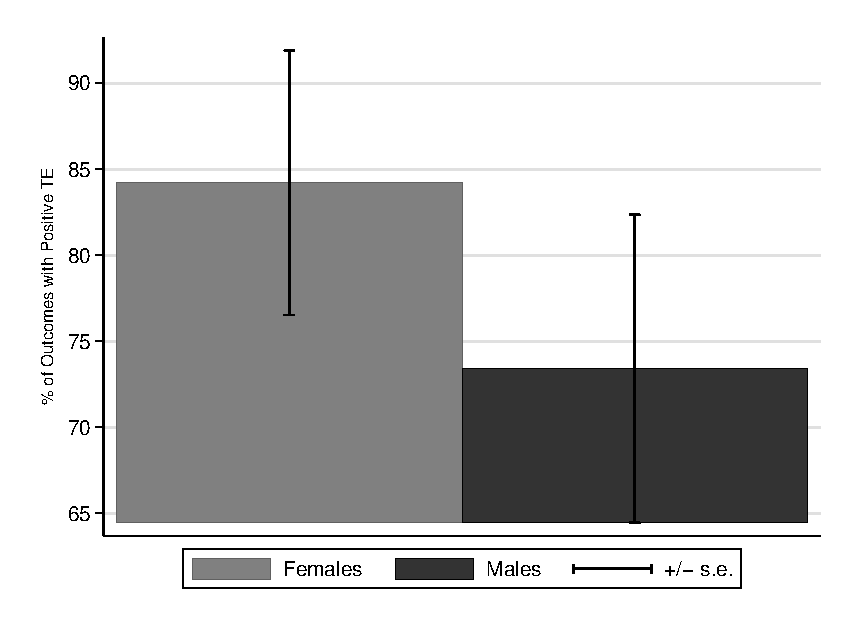
\includegraphics[width=\textwidth]{output/itt_noctrl_all.eps}
\end{subfigure}%
\begin{subfigure}[h]{0.4\textwidth}
	\centering
	\caption{Treatment vs. Next Best, Significant at 10\% Level} \label{fig:ppositive10}
		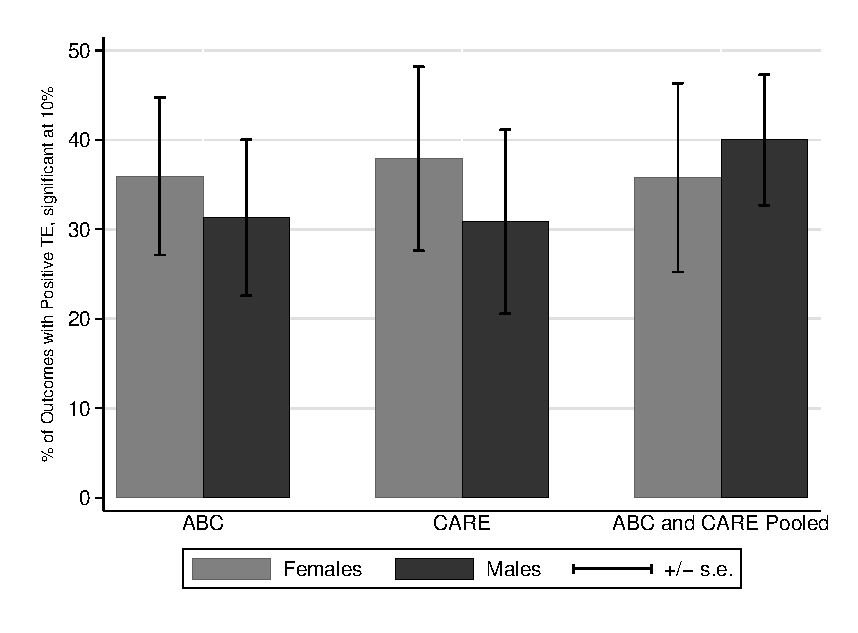
\includegraphics[width=\textwidth]{output/itt_noctrl_all_sig10.eps}
\end{subfigure}
\begin{subfigure}[h]{0.4\textwidth}
		\centering
		\caption{ Treatment vs. Stay at Home} \label{fig:ppositivehome}
		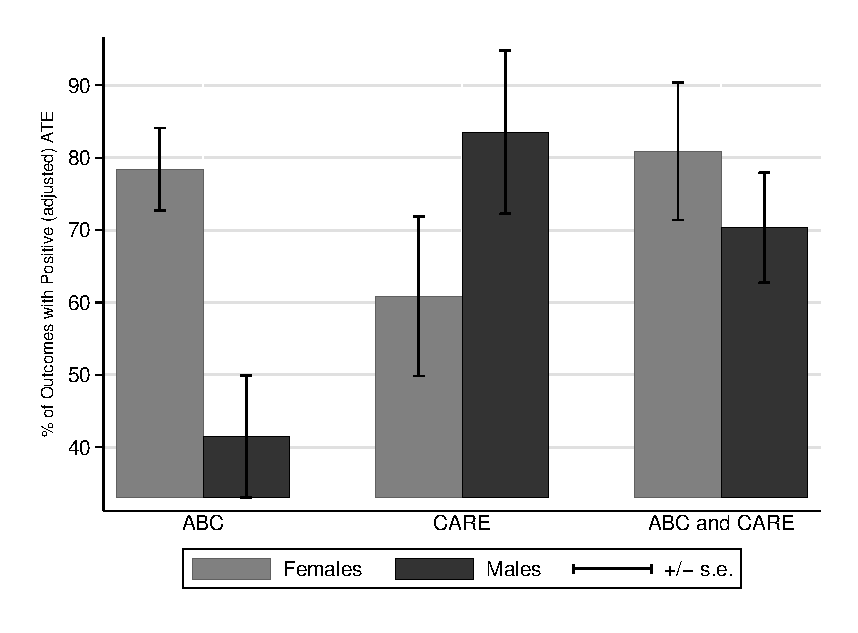
\includegraphics[width=\textwidth]{output/epan_ipw_p0_all.eps}
\end{subfigure}%
\begin{subfigure}[h]{0.4\textwidth}
	\centering
	\caption{Treatment vs. Alternative Preschool} \label{fig:ppositivealternative}
		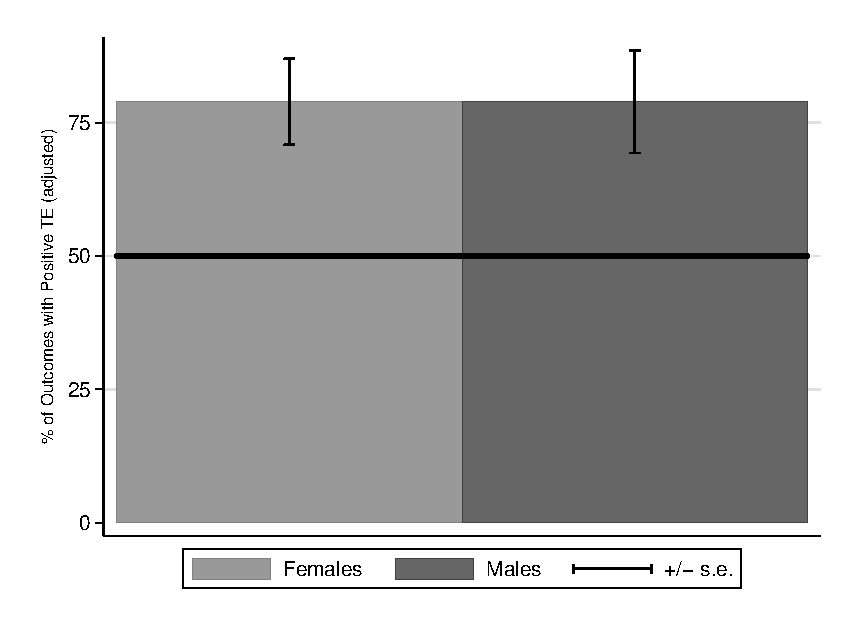
\includegraphics[width=\textwidth]{output/epan_ipw_p1_all.eps}
\end{subfigure}
\scriptsize \justify
Note: Panel (a) percentage of outcomes displaying a positive treatment effect, comparing treatment to next best. Panel (b) percentage of outcomes displaying a positive and statistically significant treatment effect (10\% significance level). Panel (c) displays the percentage of outcomes with a positive treatment effect, comparing treatment to staying at home. Panel (d) displays the percentage of outcomes with a positive treatment effect, comparing treatment to alternative childcare arrangements. Standard errors are based on the empirical bootstrap distribution. For Panel (b) we perform a ``double bootstrap'' procedure to first determine significant treatment effects at $10\%$ level and then calculate the standard error of the count.\\
\end{sidewaysfigure}

Finally, we present the estimates of the combining functions by outcome category. Figure~\ref{fig:cats-positive-significant} shows the estimated proportions that are significantly positive at the 10\% level. Consistent with the treatment effects above, control-group females tend to do better in alternative preschools than at home. This is especially true for parenting measures, IQ, education, and employment. Control-group males, on the other hand, do better at home, with more positive treatment effects in comparison to alternative preschool. The treatment effects on IQ and achievement scores, education, and employment are larger when fixing the control group to the alternative preschool. \textbf{[JJH: Report estimates here.][We moved Figure~\ref{fig:cats-positive-significant} up to be with this section.]}

\begin{figure}[H]
\centering
\caption{Positively Impacted Outcomes by Category, ABC/CARE Males and Females}\label{fig:cats-positive-significant}
\begin{subfigure}[h]{0.7\textwidth}
	\centering
	\caption{Treatment vs. Stay at Home, Significant at 10\% Level} 
		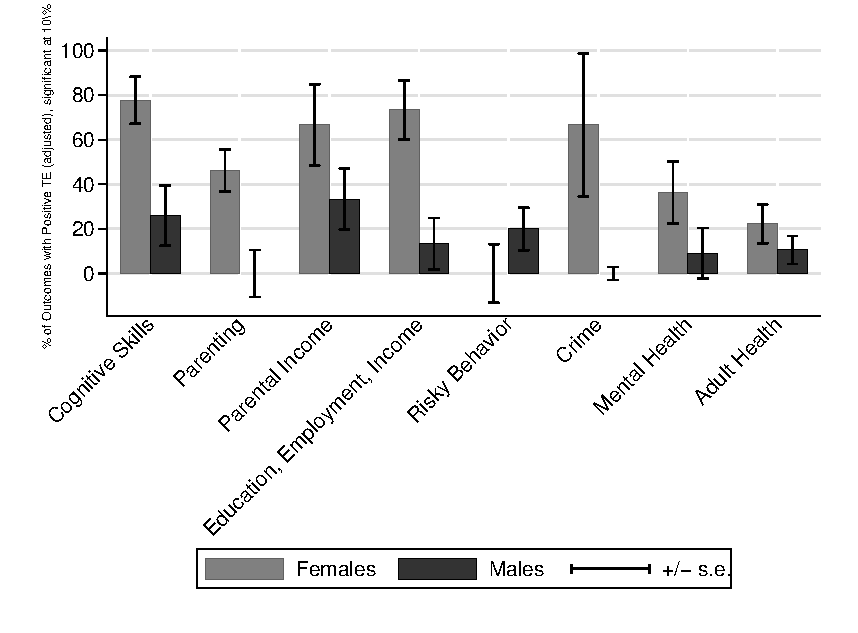
\includegraphics[width=\textwidth]{output/epan_ipw_p0_cats1_sig10.eps}
\end{subfigure}

\begin{subfigure}[h]{0.7\textwidth}
	\centering
	\caption{Treatment vs. Alternative Preschool, Significant at 10\% Level}
		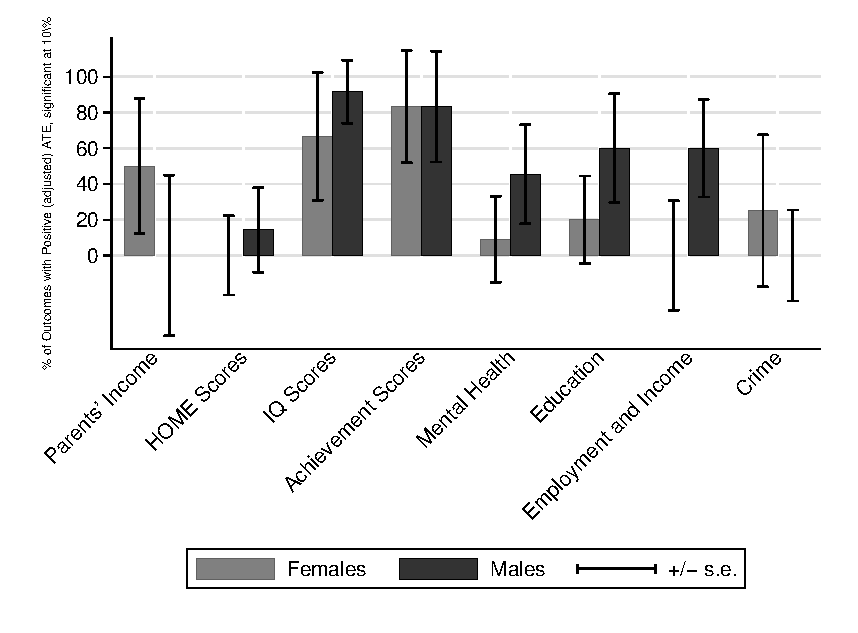
\includegraphics[width=\textwidth]{output/epan_ipw_p1_cats1_sig10.eps}
\end{subfigure}
\scriptsize \justify
Note: Panel (a) percentage of outcomes displaying a positive treatment effect, comparing treatment to next best. Panel (b) percentage of outcomes displaying a positive and statistically significant treatment effect (10\% significance level). Panel (c) displays the percentage of outcomes with a positive treatment effect, comparing treatment to staying at home. Panel (d) displays the percentage of outcomes with a positive treatment effect, comparing treatment to alternative childcare arrangements. Standard errors are based on the empirical bootstrap distribution. For Panel (b) we perform a ``double bootstrap'' procedure to first determine significant treatment effects at $10\%$ level and then calculate the standard error of the count.\\
\end{figure}



\section{Gender Differences}
\label{sec:gender-differences}
\subsection{Possible Explanations for Gender Differences}

\textbf{[We deleted the last part of this section. It was a vestige from previous drafts. This section has been updated to discuss the moderators better and connect to the literature better. We also added PARI (Parental Attitude Research Instrument) to the parenting category. Finally, we added maternal locus of control as a moderator (the closest we had to depression). It is striking to compare the treatment and control plots aggregating over all outcomes (see Figure~\ref{fig:proportion-mlocus}).]}

This section discusses the factors producing gender differences. A major determinant is the choice of the alternative child care arrangements. 
Estimated treatment effects are very similar across genders for treatment compared to those staying at home full time. Males benefit much more from treatment relative to alternative preschools compared to their benefits from treatment relative to staying at home. This result is consistent with previous research that shows (i) stark gender differences resulting from attending low quality childcare \citep{Kottelenberg-Lehrer_2014_Gender-Effects,Baker_Gruber_Milligan_2015_Noncog_Defects}; and (ii) that females are less sensitive to uncertain environments (see, e.g., \citealp{Autor-etal_2015_Family-Disadvantage}).

In the Section~\ref{sec:introduction} (Figure~\ref{fig:proportion}), we show the proportion of outcomes, by outcome category, for which the males exceed the females. Here, we further divide the control group by the alternative setting and both the treatment and control groups by father present, an important moderator. Figure~\ref{fig:proportion-altpre} shows the proportions dividing by alternative setting. The males who stay at home do better than the females in cognitive and parenting measures, employment, and across all outcomes. Unlike the males who attend alternative preschool, the males who stay at home have similar crime outcomes as the females. Given the prominence of the male criminal activity, this finding highlights the magnitude of harm caused by low-quality alternative preschools for the males. 

\begin{figure}[H]
\centering
\caption{Proportion of Outcomes Males $>$ Females, by Outcome Category, Dividing by Alternative Setting}
\label{fig:proportion-altpre}
	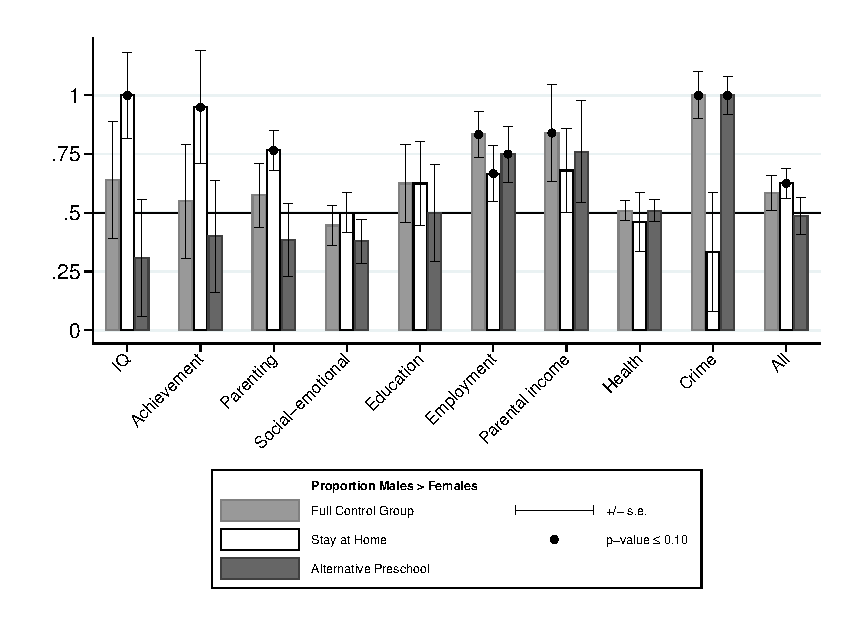
\includegraphics[width=\textwidth]{output/gendergaps-control-moderated-altpre}
\footnotesize \justify
Note: These plots show the proportion of outcomes, by outcome category, for which the males' mean is larger than the females' mean. The standard errors and the $p$-values are computed using 100 bootstraps. The $p$-values are one-sided and test the null hypothesis that the proportion of outcomes is greater than $\frac{1}{2}$ The crime outcomes are all coded so that a higher value indicates more criminal activity. All other outcome categories have higher values corresponding to socially desirable outcomes. 
\end{figure}

Next, we report these proportions by father present (Figure~\ref{fig:proportion-fhome}). Father's presence interacted with treatment favors males for IQ, parenting, and health measures. Males in the control group do better when the father is absent in education and employment. This indicates that treatment complements the home environment for males more than for females. 

\begin{figure}[!htbp]
\centering
\caption{Proportion of Outcomes Males $>$ Females, by Outcome Category, Dividing by Father Present}
\label{fig:proportion-fhome}
\begin{subfigure}[h]{0.7\textwidth}
	\centering
	\caption{Control Group}
	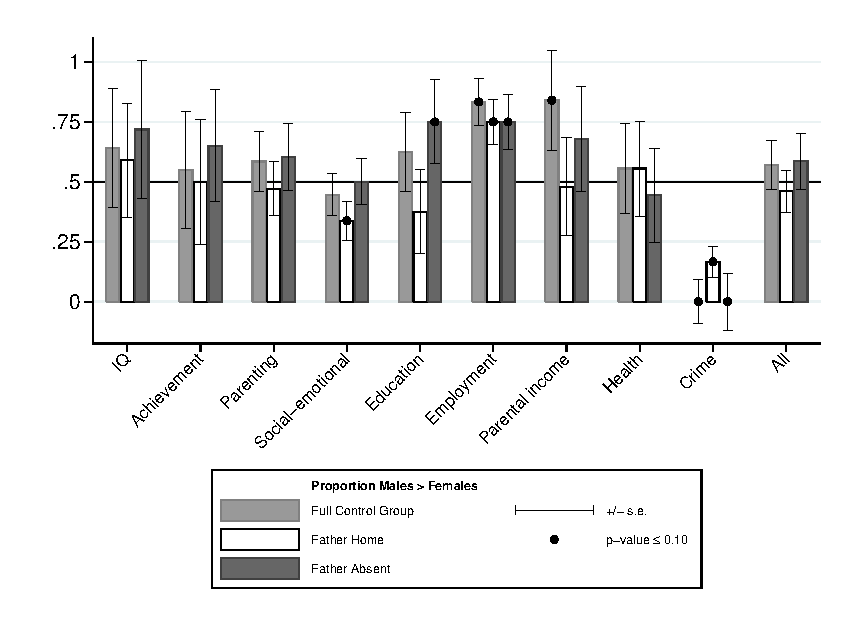
\includegraphics[width=\textwidth]{output/gendergaps-control-moderated-fhome}
	\end{subfigure}
	
\begin{subfigure}[h]{0.7\textwidth}
	\centering
	\caption{Treatment Group}
	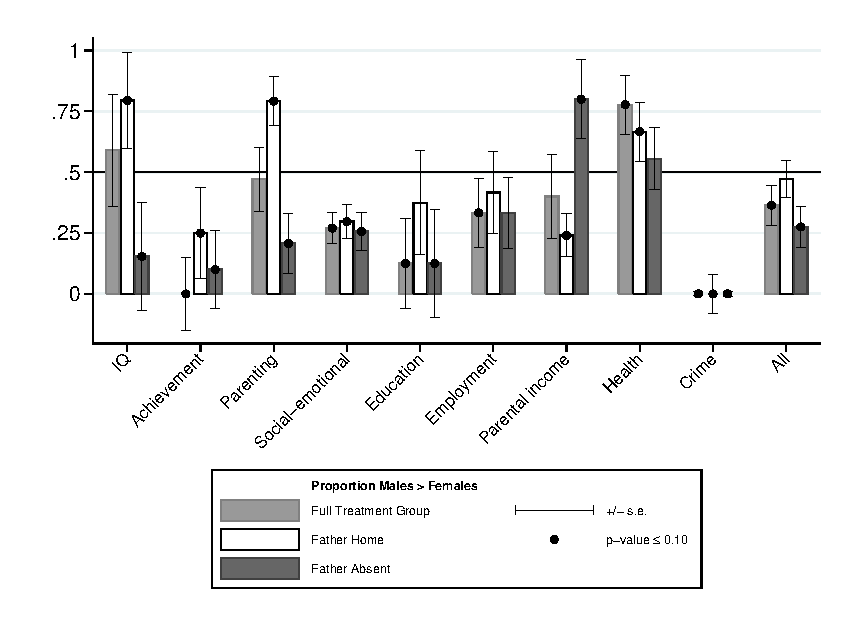
\includegraphics[width=\textwidth]{output/gendergaps-treatment-moderated-fhome}
	\end{subfigure}
\footnotesize \justify
Note: These plots show the proportion of outcomes, by outcome category, for which the males' mean is larger than the females' mean. The standard errors and the $p$-values are computed using 100 bootstraps. The $p$-values are one-sided and test the null hypothesis that the proportion of outcomes is greater than $\frac{1}{2}$ The crime outcomes are all coded so that a higher value indicates more criminal activity. All other outcome categories have higher values corresponding to socially desirable outcomes. 
\end{figure}

Another measure of home environment maternal locus of control, which is measured when the subjects were 1.5 years old.\footnote{We define internal locus of control as scoring below the sample mean and an external locus of control as scoring at or above the sample mean. See \citet{Rotter_1966_PMGaA}.} An internal locus of control indicates feeling in control of future outcomes, including those related to child rearing. In contrast, an external locus of control indicates feeling that outside forces determine future outcomes (e.g. luck). Figure~\ref{fig:proportion-mlocus} shows this exercise. In the control group, an internal locus of control leads to better outcomes for males across all outcome categories except health. Another way to state this is that males are more hurt by their mothers having an external locus of control than are females. Although locus of control does not necessarily measure depression, this finding corresponds with \citet{Beeghly-etal_2017_IMHJ}, who find that increased maternal depression lead to worse outcomes for young males relative to females. 

\begin{figure}[!htbp]
\centering
\caption{Proportion of Outcomes Males $>$ Females, by Outcome Category, Dividing by Maternal Locus of Control}
\label{fig:proportion-mlocus}
\begin{subfigure}[h]{0.7\textwidth}
	\centering
	\caption{Control Group}
	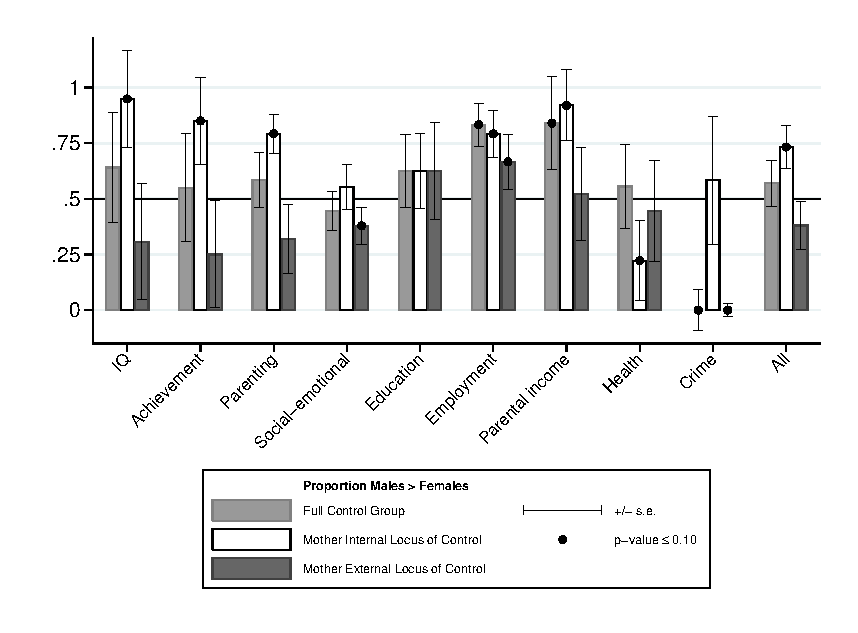
\includegraphics[width=\textwidth]{output/gendergaps-control-moderated-mlocus}
	\end{subfigure}
	
\begin{subfigure}[h]{0.7\textwidth}
	\centering
	\caption{Treatment Group}
	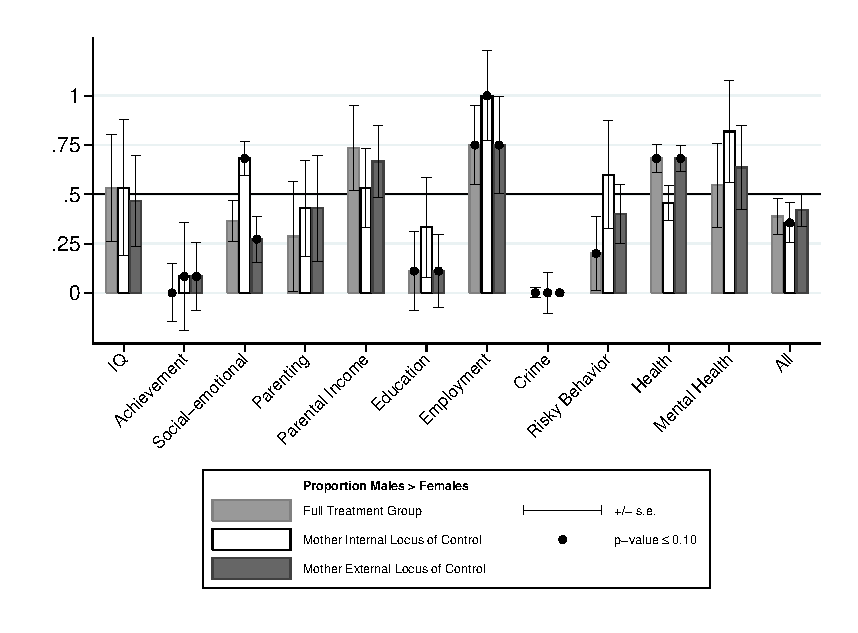
\includegraphics[width=\textwidth]{output/gendergaps-treatment-moderated-mlocus}
	\end{subfigure}
\footnotesize \justify
Note: These plots show the proportion of outcomes, by outcome category, for which the males' mean is larger than the females' mean. The standard errors and the $p$-values are computed using 100 bootstraps. The $p$-values are one-sided and test the null hypothesis that the proportion of outcomes is greater than $\frac{1}{2}$ The crime outcomes are all coded so that a higher value indicates more criminal activity. All other outcome categories have higher values corresponding to socially desirable outcomes. 
\end{figure}

Maternal locus of control moderates the treatment outcomes differently. Regardless of locus of control males do not do much better than their female counterparts. The exception is for health outcomes, in which the pattern of boys with mothers with external loci of control outperform those with mothers with internal loci of control. Aggregating across outcomes, we can see that maternal locus of control does not moderate the males' outcomes if they attend ABC/CARE as it does if they are in the control group. 





\section{Conclusion}
\label{sec:conclusion}
\textbf{[JJH: Need to point out consistency with the literature.][We edited the conclusion to connect more with the literature.]}

Although several studies of early childhood education report effects by gender, they do not consider two important factors. The first factor is that there can be gender gaps before treatment that are then changed after treatment. We find that control-group males tend to do better than the control-group females, especially in education and employment outcomes. After treatment, most these gaps are narrowed or reversed. This corresponds with the finding that a larger proportion of the treatment effects are positive and significant for females than for males. ABC/CARE, in addition to improving select individual outcomes, also narrowed the male-female gap in important categories of outcomes. 

The second factor to consider is the alternative setting. We find that lower quality preschools are especially detrimental for boys. This connects to previous work that finds boys to be more vulnerable early in life than girls \citep{golding2016psychology}. Boys similarly are more harmed by unstable home environments (measured by father present and maternal locus of control) than girls. 



\clearpage
\singlespacing
\bibliography{heckman}
\bibliographystyle{chicago}

\end{document}
